%https://www.overleaf.com/9980828whgsqyqzhjkx#/36673404/

\documentclass[a4paper]{article}

%% Language and font encodings
\usepackage[ngerman]{babel}
\usepackage[utf8x]{inputenc}
\usepackage[T1]{fontenc}

%% Sets page size and margins
\usepackage[a4paper,top=3cm,bottom=4cm,left=2.5cm,right=2.5cm,marginparwidth=1.75cm]{geometry}

%% Useful packages
\usepackage{amsmath}
\usepackage{graphicx}
\usepackage{float}
%\usepackage[colorinlistoftodos]{todonotes}
\usepackage[colorlinks=true, allcolors=black]{hyperref}

\title{Belegarbeit Multimediale Signalverarbeitung\\Spektrumanalysator}
\author{Toni Barth, Max Haarbach}

\begin{document}
\begin{titlepage}
\clearpage\maketitle
\thispagestyle{empty}
\end{titlepage}

%\begin{abstract}
%Your abstract
%\end{abstract}

\newpage
\tableofcontents
\newpage
\listoffigures
\newpage
\section{Einführung}\label{sec:einführung}

\subsection{Aufgabenstellung}\label{subsec:aufgabenstellung}

SA Spektrumanalysator (Oszilloskop): Applikation ermöglicht die Visualisierung und Analyse von Signalen im Frequenzbereich
\begin{itemize}
  \item Funktionaler Umfang
  \begin{itemize}
    \item ein Eingang, veränderbare Zeitbereich/ Frequenzbereich und Amplitude, Frequenzband des Signals über Bandbegrenzung einstellbar, Spektrum, Spektrogramm
  \end{itemize}
  \item Simulation der Darstellungsformen, Berechnungen und Filterfunktionen (Spektrogram ohne lib umsetzen, selber coden!)
  \item Erzeugen verschiedener Testsignale (z.B. Rauschen, Sinus, Musikstück)
  \item Darstellung und Vergleich (Zeit- und Frequenzbereich) sowie Veränderung Parameter/ Algorithmen/ Umsetzung, Einfluss der FFT-Auflösung (Spektralkomponenten)
  \begin{itemize}
    \item Signale im Zeit- und Frequenzbereich (Spektrogram und Spektrum)
    \item FFT-Auflösung/ Signallänge/ Fensterung
  \end{itemize}
  \item Validierung korrekter Funktionsweise (stimmt angezeigte Frequenz?, kontinuierliche Darstellung, usw.)
\end{itemize}

\subsection{Ziel der Arbeit}\label{subsec:zielDerArbeit}

Das Ziel der Arbeit ist es, die Funktionsweise der auditiven Signalverarbeitung nicht nur zu verstehen, sondern in ihren Grundzügen auch selber Anwenden zu können. Zu diesem Zweck sollen möglichst viele Funktionen des Programmes selbst implementiert werden. Hierbei wird sowohl der Aufbau eines Signals, aber auch das Zusammenführen dieser, das Analysieren und verändern (bspw. durch Resampling, Downmixing etc) vermittelt und angewendet. Das Ziel der Arbeit und des Programmes an sich ist es, ein Programm zur Verfügung zu stellen, welche die oben genannten Anforderungen umsetzt.

\subsection{Anwendungsfälle}\label{subsec:anwendungsfälle}

Dieses Programm ist hilfreich, um sich ein Audiosignal visualisiert darstellen zu lassen. Man kann hierbei untersuchen, welche Frequenzen in einem Audiosignal der Wahl (oder in generierten Testsignalen) besonders häufig vorhanden sind / besonders laut sind und so einen Eindruck über das Signal bekommen, ohne es sich anhören zu müssen. Außerdem kann man gezielt Frequenzen herausfiltern und sich das Ergebnis ohne diese Frequenzen visualisieren lassen. Zudem kann man sich Testsignale visualisieren lassen, um Erfahrung darüber zu gewinnen, wie typische Signale aussehen.

\newpage
\section{Anforderungsanalyse}\label{sec:anforderungsanalyse}

\subsection{Projektintension}\label{subsec:projektintension}

Der Zweck des Projektes besteht darin, sich mit der digitalen Signalverarbeitung in informationstechnologischer Hinsicht auseinanderzusetzen und dessen Verständnis zu fördern. Vor allem die Stichwörter Fast-Fourier-Transformation und Filterung sowie Manipulation stellen hier wichtige Bestandteile dar. Zudem bietet es die Möglichkeit, herauszufinden, wie Diagramme und andere Darstellungen durch Programme realisiert werden können.

\subsection{Funktionale Anforderungen}\label{subsec:funktionaleAnforderungen}

Folgende funktionale Anforderungen können der Aufgabenstellung entnommen werden:
\begin{itemize}
  \item ein Eingang (Testsignal, Audiodatei)
  \item veränderbarer Zeitbereich
  \item veränderbarer Frequenzbereich
  \item veränderbare Amplitude
  \item einstellbare Bandbegrenzung des Eingangsignals
  \item Spektrum (Frequenzbereich des Signals)
  \item Spektrogramm (Frequenzbereich über Zeit hinweg)
\end{itemize}

\subsubsection{Weitere Anforderungen}

Zu den Anforderungen an das Projekt, die sich nicht direkt in Funktionalitäten äußern, gehören:
\begin{itemize}
  \item Simulation von:
  \begin{itemize}
    \item Darstellungen
    \item Berechnungen
    \item Filterfunktionen
  \end{itemize}
  \item Erzeugen von Testsignalen
  \item Vergleich von zwischen den unterschiedlichen Darstellungeformen
  \item Vergleich von Darstellungen untereinander mit unterschiedlichen Parametern und Algorithmen
  \item Validierung der korrekten Funktionsweise
\end{itemize}

\subsubsection{Abgrenzung des Produkts}

Da der Bereich der digitalen Signalverarbeitung sehr groß ist, besteht die Notwendig zu erläutern, welche Funktionen nicht vom Programm gefordert sind. Dazu zählen sowohl die akustische Ausgabe der Signale als auch die Speicherung von neuen erzeugten Signalen, obwohl diese Punkte auch sehr interessant für Analysen sein würden.\\
Außerdem ist es im Hinblick des Aufwandes nicht angemessen, alle möglichen Eingabeparameter auch dem Nutzer zur Verfügung zu stellen, da sich meist die Ausgabe nur minimal ändert. Im Gegenzug wird versucht, für diese nicht festlegbaren Parameter möglichst die besten Werte zu wählen.\\
Zuletzt soll es auch möglich sein, eine Bandbegrenzung einstellen sowie verschiedene Zeitbereiche betrachten zu können.

\subsubsection{Funktionen des Produktes}

Das Programm soll im ersten Schritt erst einmal Signale wie einen Sinus erzeugen können, deren Frequenz, Länge, Amplitude und Abtastrate man frei wählen kann. Daneben soll auch die Auswahl eines eigenen Audiosignals möglich sein.\\
Anschließend ist es erforderlich, dass diese dann in den verschiedenen Darstellungsformen korrekt visualisiert werden.

\subsection{Nicht-funktionale Anforderungen}\label{subsec:nicht-funktionaleAnforderungen}
%\subsubsection{Look and Feel}
%\subsubsection{Usability}
%\subsubsection{Barrierefreiheit}
\subsubsection{Performance}

Das Endprodukt soll in der Leistung um ein Vielfaches schneller als Echtzeit sein, d.h. die Analyse eines 3-minütigen Audiosignals soll möglichst nur wenige Sekunden dauern. Das selbe gilt auch für die Anwendung von Filtern oder das Verändern von Analyse-Parametern. Zudem soll die Verwendung der Bedienoberfläche flüssig ablaufen, es sollten also keine Aussetzer oder Hänger aufgrund zu hoher Hintergrundaktivität auftreten.

%\subsubsection{Skalierbarkeit/Erweiterbarkeit}
%\subsubsection{Übersicht aller Anforderungen}

\newpage
\section{Ähnliche Anwendungen}\label{sec:ähnlicheAnwendungen}

\subsection{Sonic Visualiser}\label{subsec:sonicVisualiser}
"`Sonic Visualiser"' ist eine kostenlose Software, mit der viele verschiedene Darstellungen von Audiosignalen möglich sind.
So können Audiodateien der Formate WAV, Ogg und MP3 geladen werden, deren Schwingungsverlauf im Zeitbereich dann betrachtet werden kann. Zudem kann aber auch das Spektrum, Spektrogramm und weitere Diagramme dargestellt werden, die durch verschiedene Parameter beeinflusst und verändert werden können. Diese wiederum können unterschiedlich angeordnet und auch überlagert werden, um so Zusammenhänge zwischen ihnen besser zu erkennen.\\
Zur Abrundung des Ganzen besteht außerdem die Möglichkeit, die Audiodatei wiederzugeben während sich ein Cursor entsprechend über die Diagramme bewegt.
\vspace{2em}
\begin{figure}[H]
    \centering
    \begin{minipage}{0.35\textwidth}
        \centering
        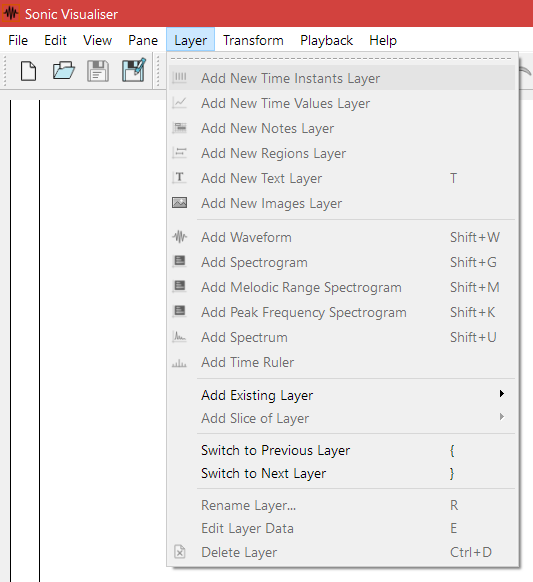
\includegraphics[width=1.0\textwidth]{Sonic_Layers.png}
        \caption{Verschiedene Ebenen in "`Sonic Visualiser"'}
    \end{minipage}
\end{figure}
\noindent
In dieser Abbildung sieht man, welche verschiedenen Layer man auswählen kann, die im den Diagrammbereich dargestellt werden sollen.
\vspace{2em}
\begin{figure}[H]
    \centering
    \begin{minipage}{1.0\textwidth}
        \centering
        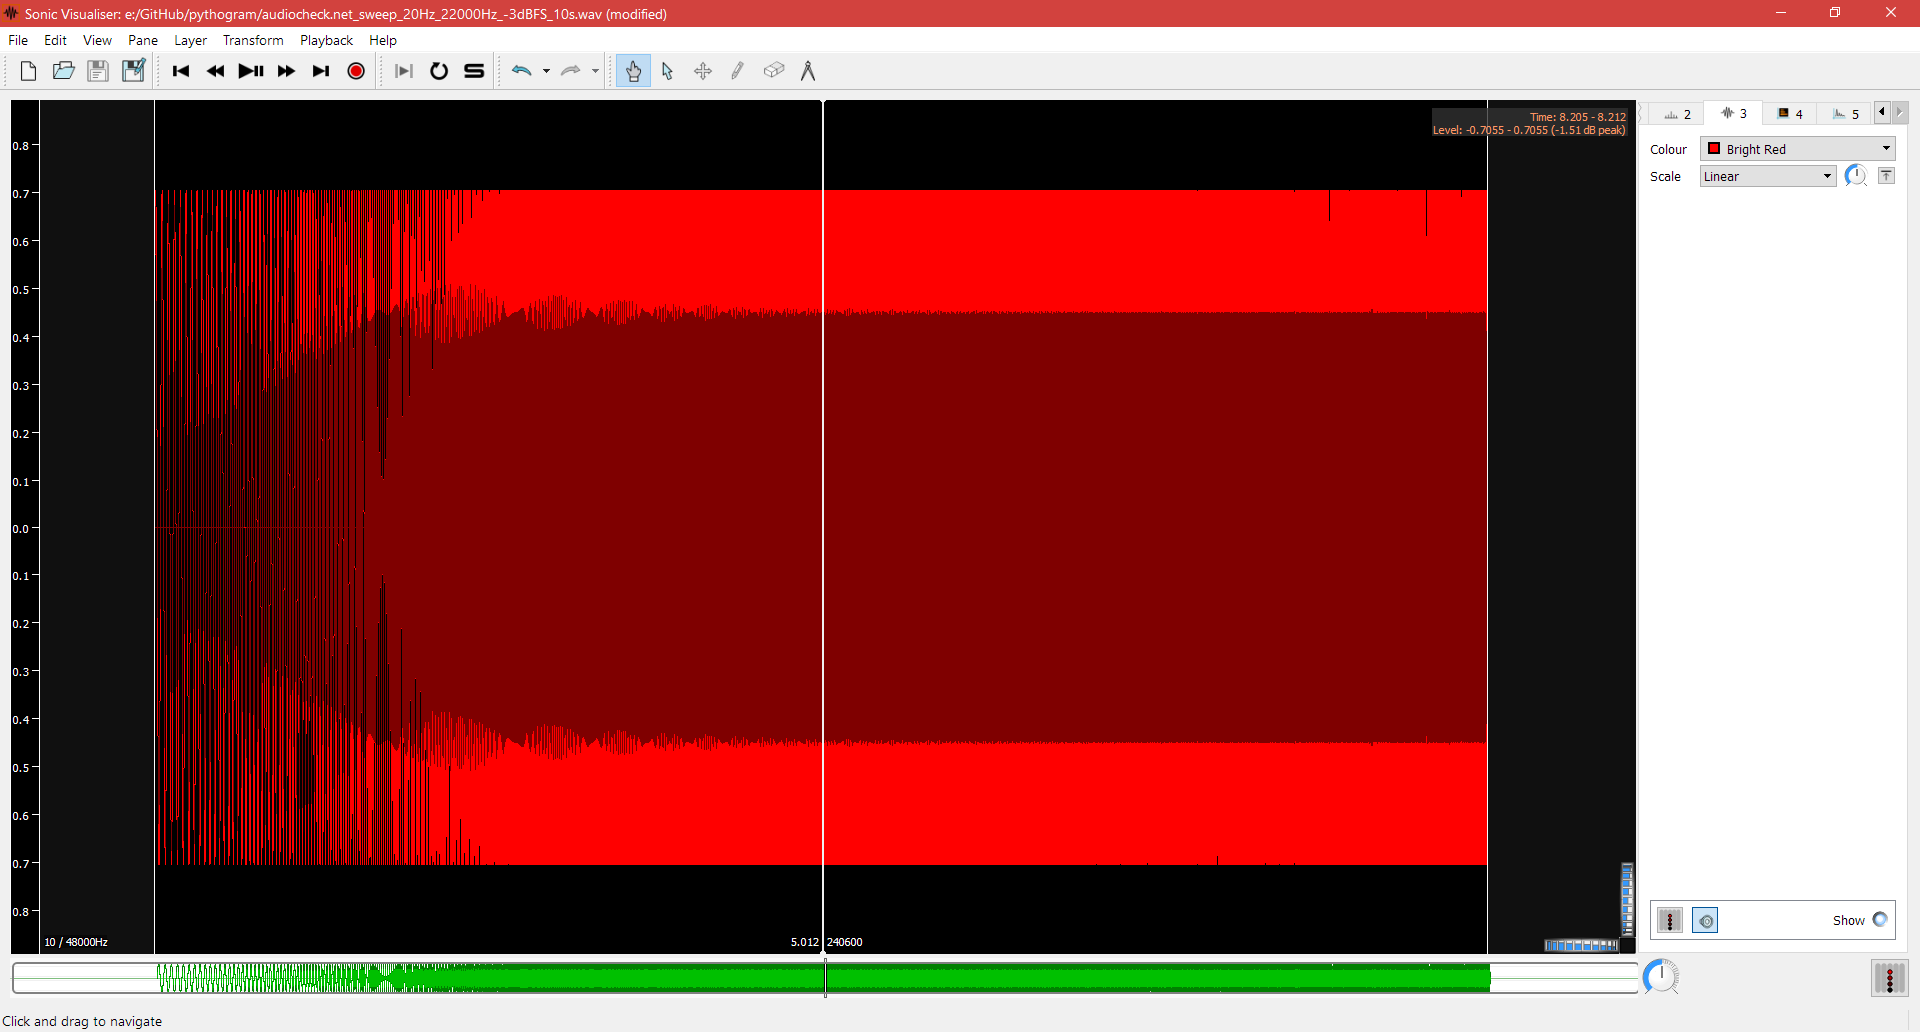
\includegraphics[width=0.7\textwidth]{Sonic_Sine_Sweep_Wave.png}
        \caption{Wellenform eines steigenden Sinus in "`Sonic Visualiser"'}
    \end{minipage}
\end{figure}
\noindent
Bei der Darstellung der Wellenform kann man angeben, in welcher Farbe die Wellen und welcher Skalierung die Amplitude dargestellt werden soll.
\vspace{2em}
\begin{figure}[H]
    \centering
    \begin{minipage}{1.0\textwidth}
        \centering
        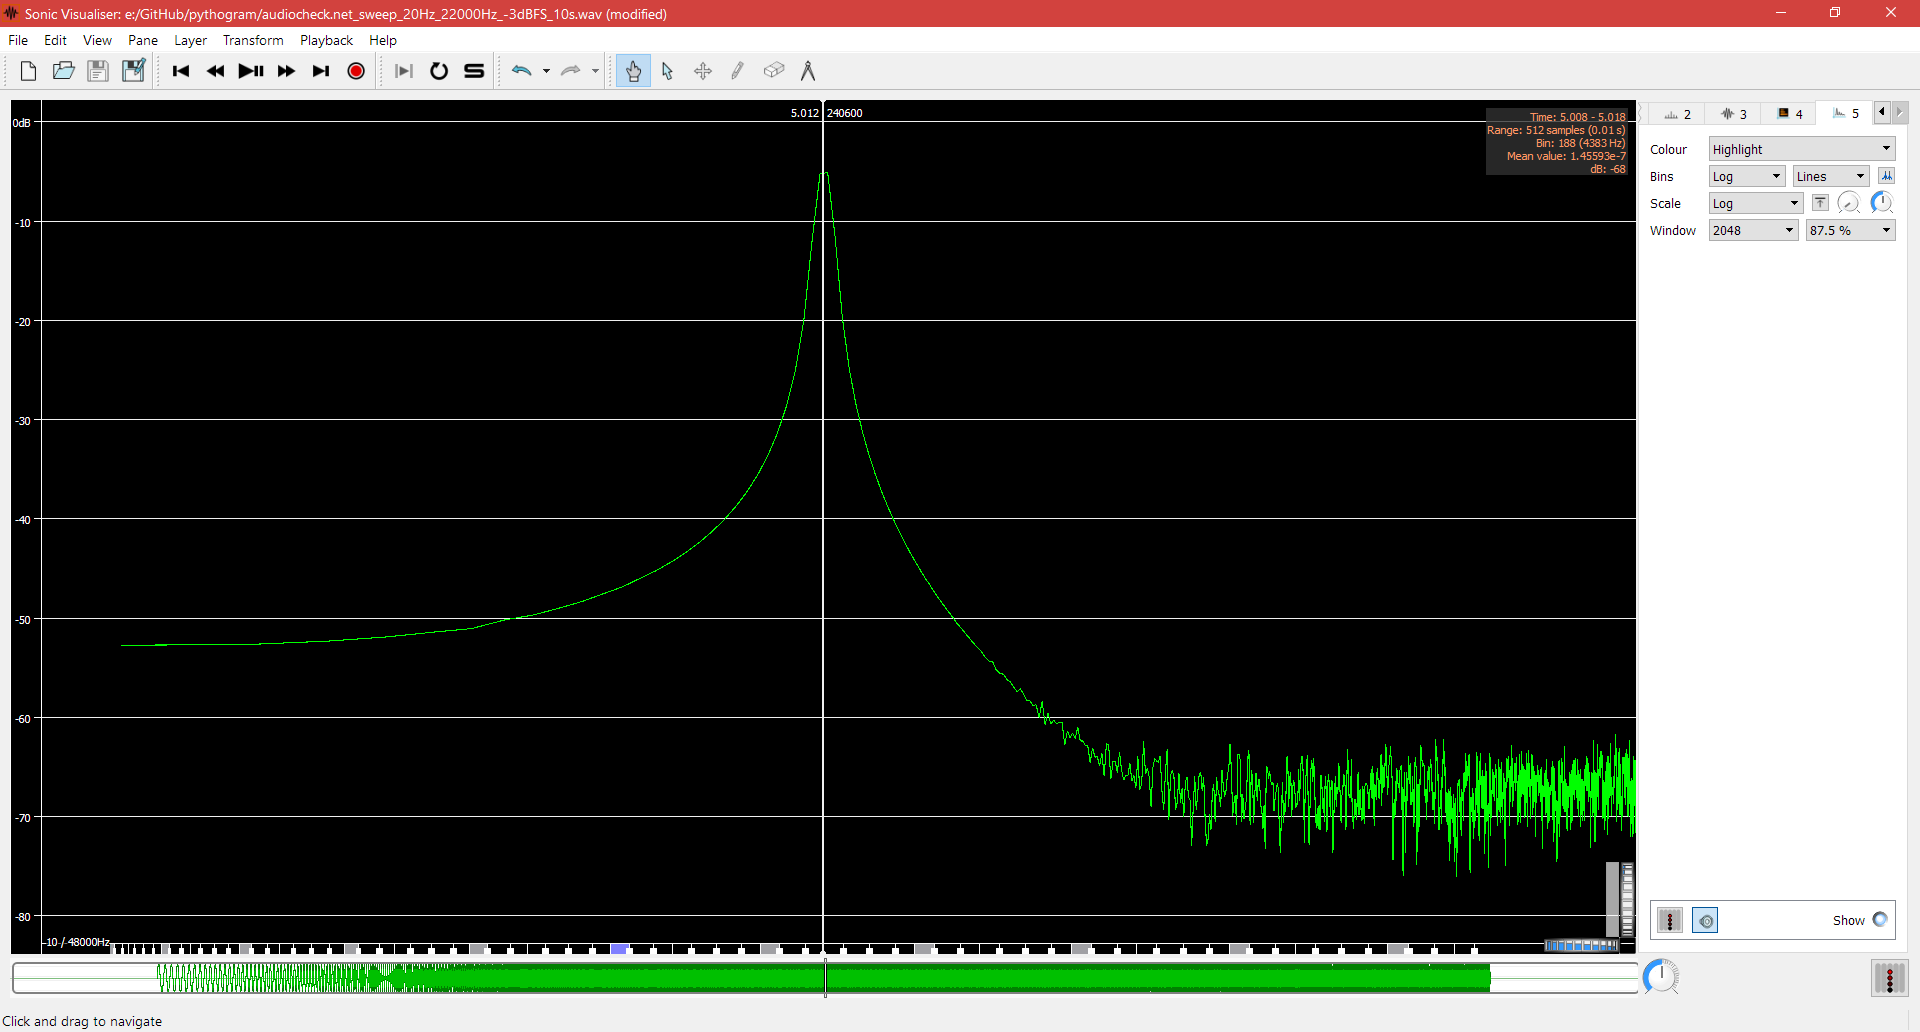
\includegraphics[width=0.8\textwidth]{Sonic_Sine_Sweep_Spectrum_on_5s.png}
        \caption{Spektrum eines steigenden Sinus bei ca 5 s in "`Sonic Visualiser"'}
    \end{minipage}
\end{figure}
\noindent
Beim Spektrum kann man wiederum die Farbe einstellen und in welcher Skalierung die Frequenz und Amplitude dargestellt werden soll. Außerdem ist die FFT-Auflösung bzw. Fensterung ein wichtiger Parameter. Je nach dem, an welcher Stelle des Signals man den Cursor positioniert hat, wird das Spektrum des Signals zu diesem Zeitpunkt dargestellt, was vor allem bei Wiedergabe des Signals interessant ist, da der Cursor der Wiedergabe folgt und somit immer das aktuelle Spektrum dargestellt wird.
\vspace{2em}
\begin{figure}[H]
    \centering
    \begin{minipage}{1.0\textwidth}
        \centering
        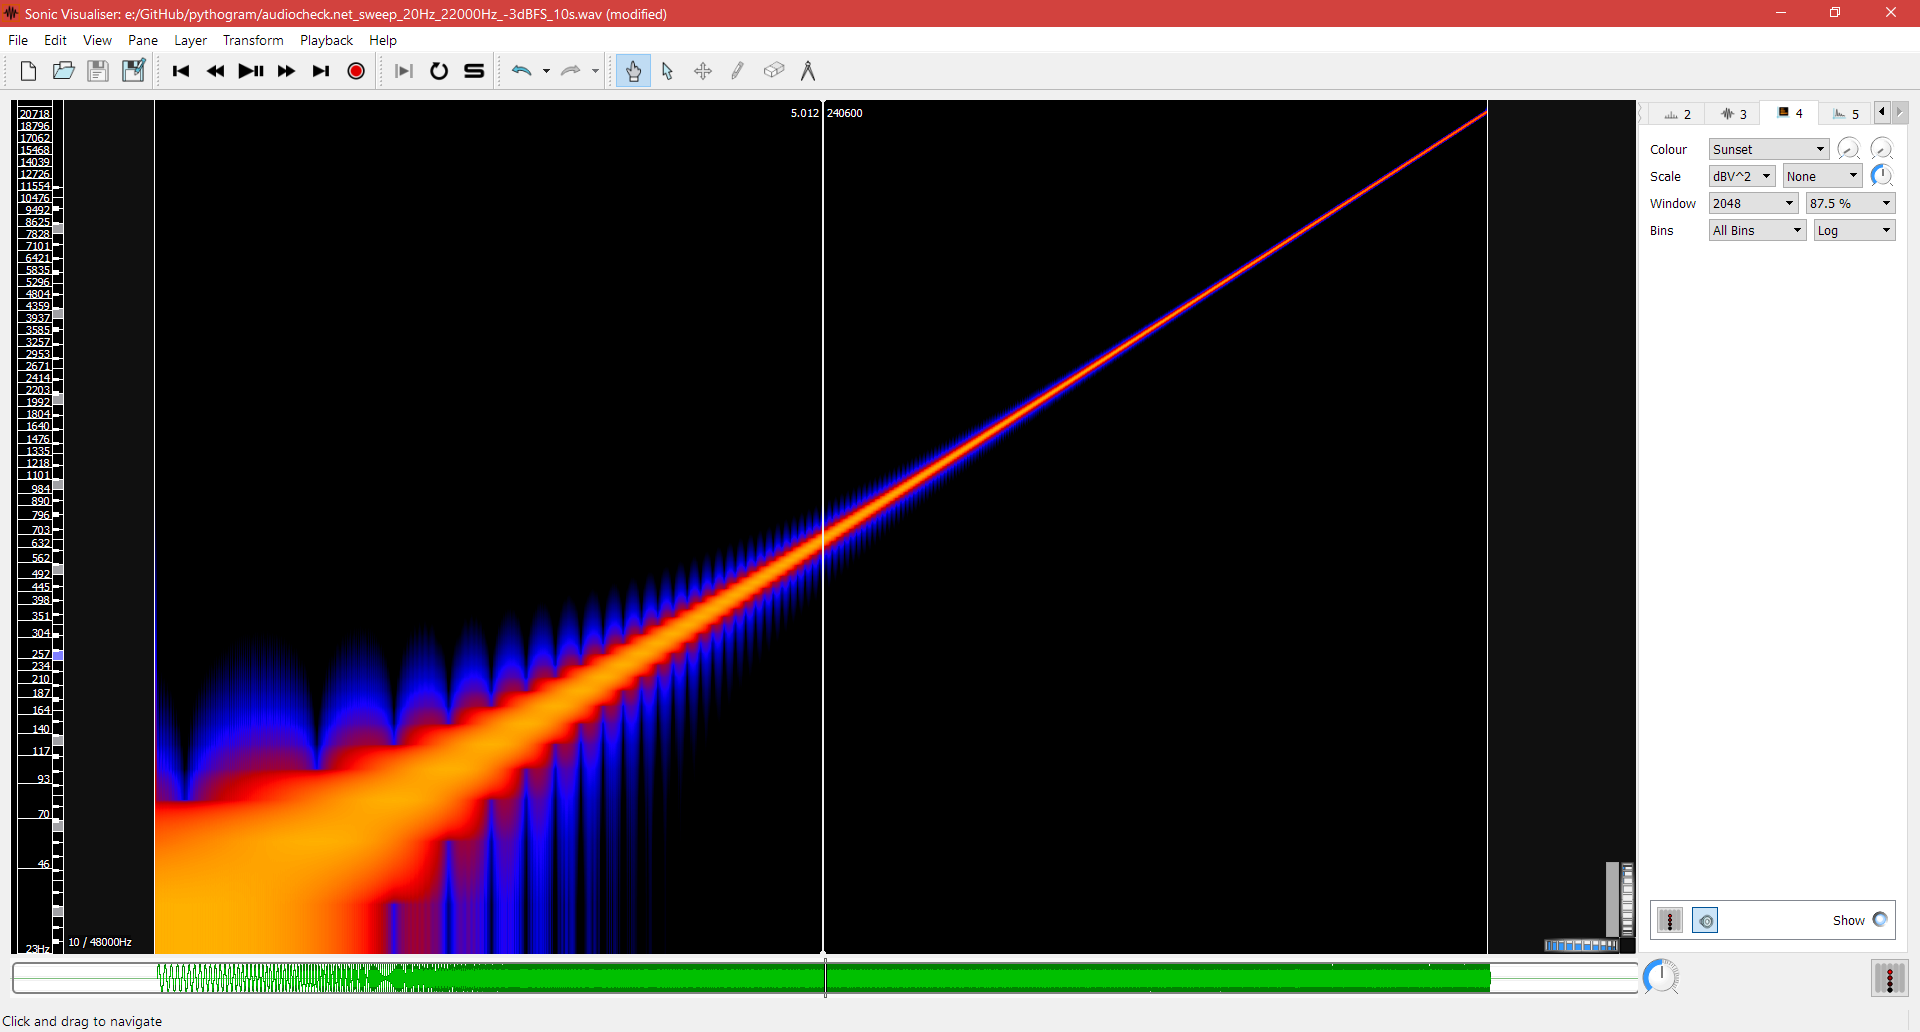
\includegraphics[width=0.8\textwidth]{Sonic_Sine_Sweep_Spectrogram.png}
        \caption{Spektrogramm eines steigenden Sinus in "`Sonic Visualiser"'}
    \end{minipage}
\end{figure}
\noindent
Auch beim Spektrogramm kann die Farbe gewählt und ähnliche Parameter wie bei Spektrum eingestellt werden, da ein Spektrogramm im Endeffekt eine Zusammensetzung von mehreren kleinen Spektren ist. Daher kann hier auch die Skalierung der Amplitude und der Frequenzachse sowie die FFT-Auflösung verändert werden.
\vspace{2em}
\begin{figure}[H]
    \centering
    \begin{minipage}{1.0\textwidth}
        \centering
        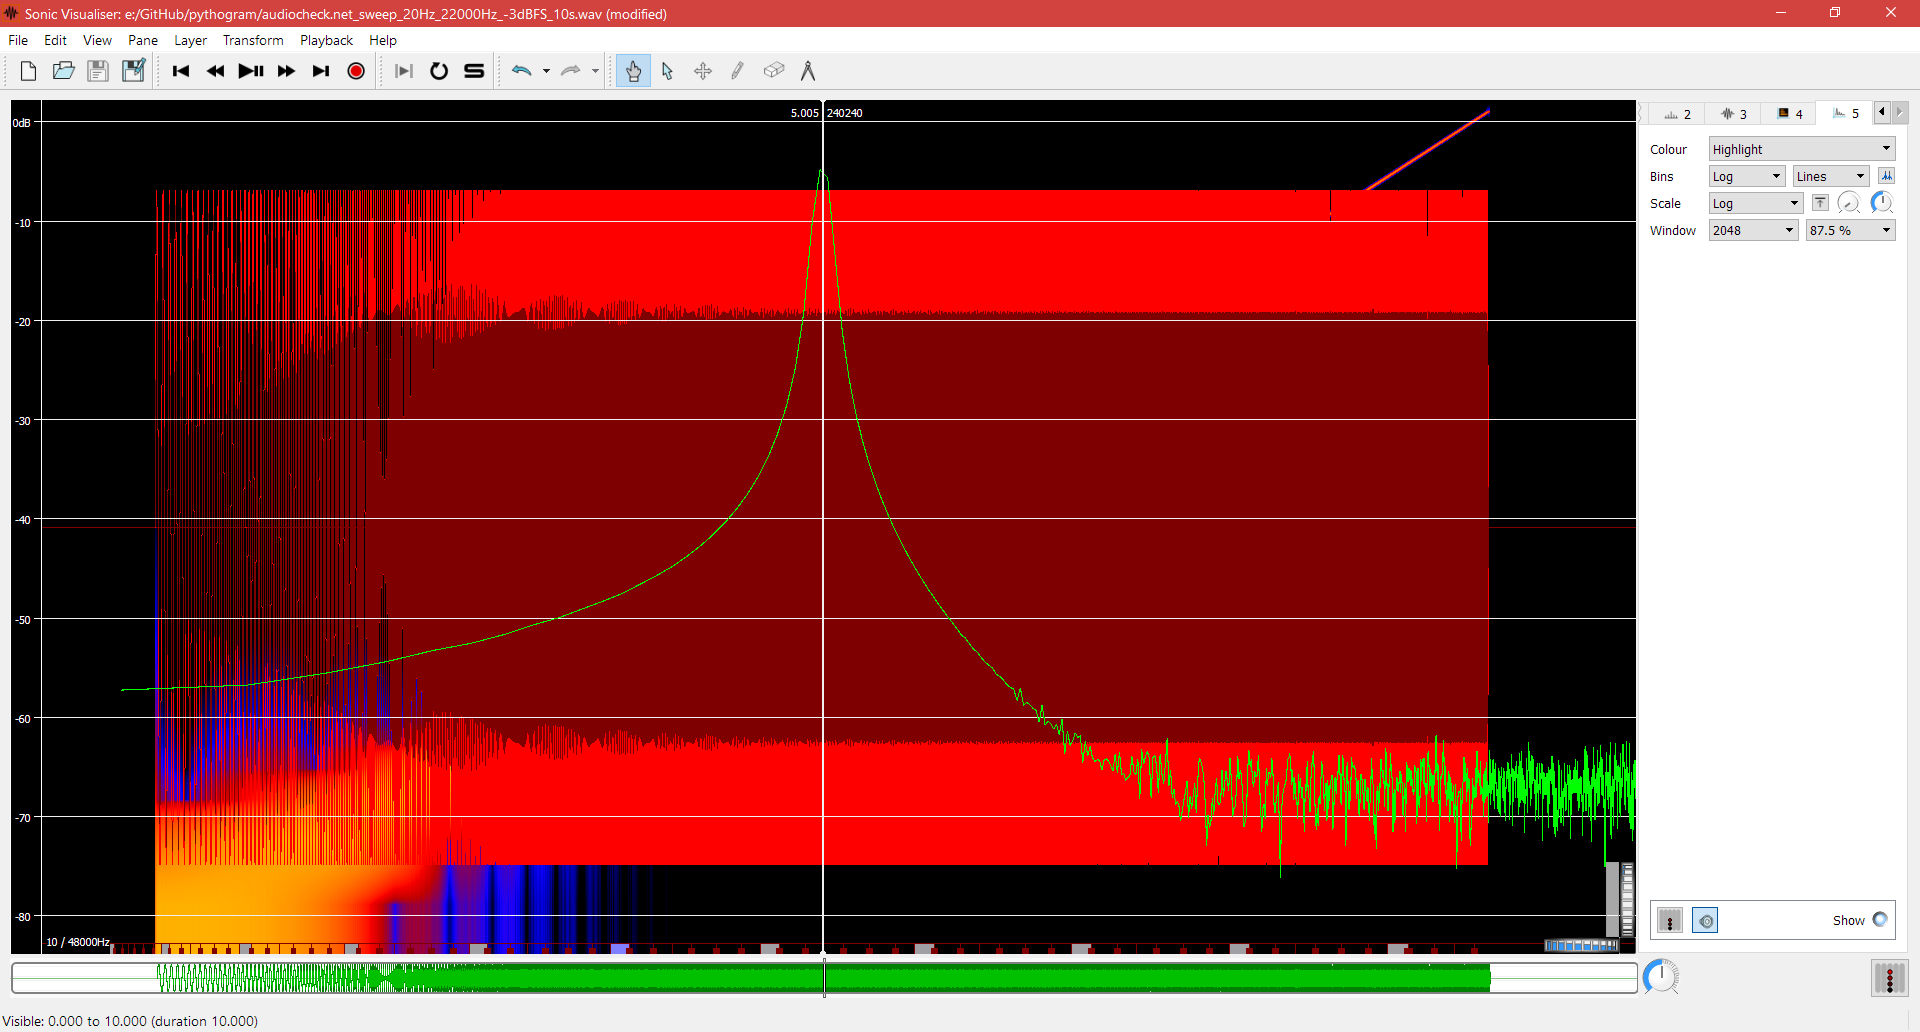
\includegraphics[width=0.8\textwidth]{Sonic_Sine_Sweep_overlay.png}
        \caption{Überlagerung mehrerer Diagramme eines steigenden Sinus in "`Sonic Visualiser"'}
    \end{minipage}
\end{figure}
\noindent
Hier sieht man die vorigen Diagramme alle überlagert. Man kann diese aber auch in mehreren separaten Bereichen anordnen können, z. B. Wellenform und Spektrum überlagert in der oberen Hälfte und das Spektrogramm in der unteren.
\vspace{2em}\\
Die nächsten beiden Abbildungen zeigen das Spektrogramm des Lieds "`Toms Diner"' von Susanne Vega; ein mal über dem gesamten Zeitraum und danach ca. die ersten 40 Sekunden.
\begin{figure}[H]
    \centering
    \begin{minipage}{1.0\textwidth}
        \centering
        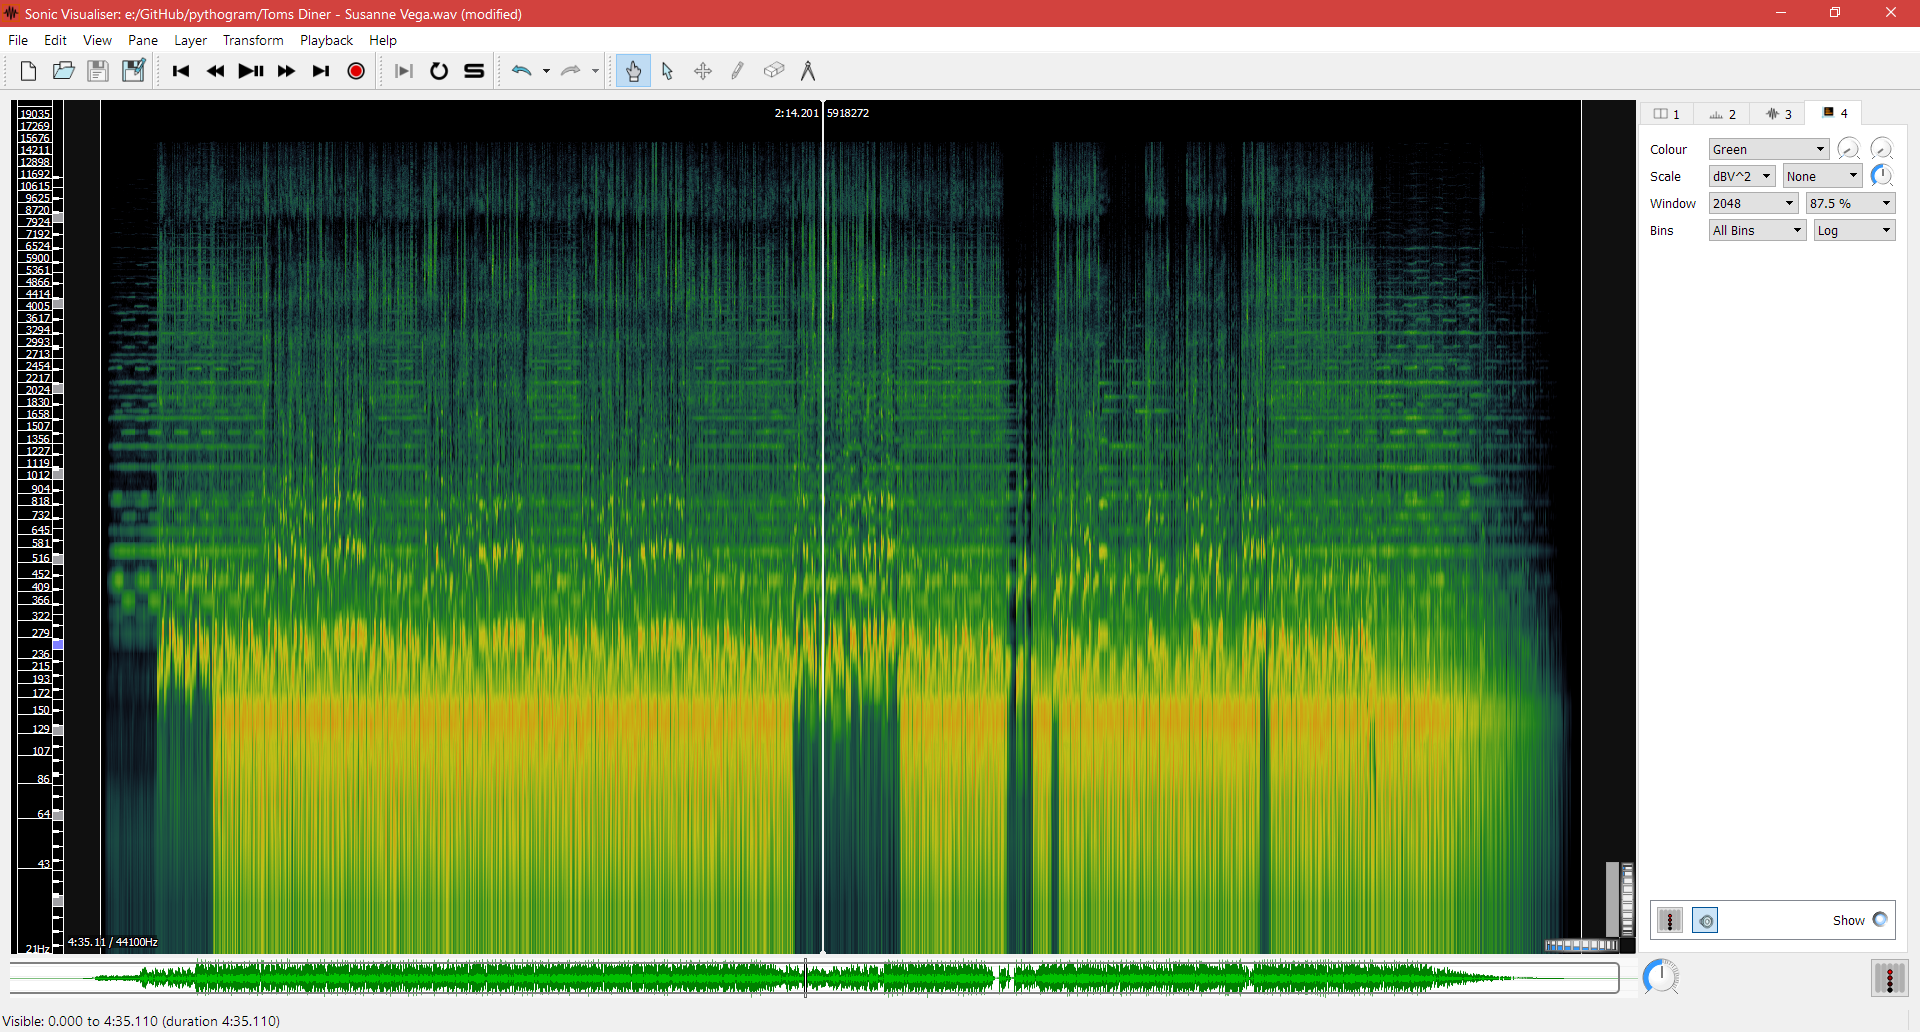
\includegraphics[width=1.0\textwidth]{Sonic_Toms_Diner_Spectrogram_all.png}
        \caption{Gesamtes Spektrogramm des Songs "`Toms Diner"' in "`Sonic Visualiser"'}
    \end{minipage}
\end{figure}
\begin{figure}[H]
    \centering
    \begin{minipage}{1.0\textwidth}
        \centering
        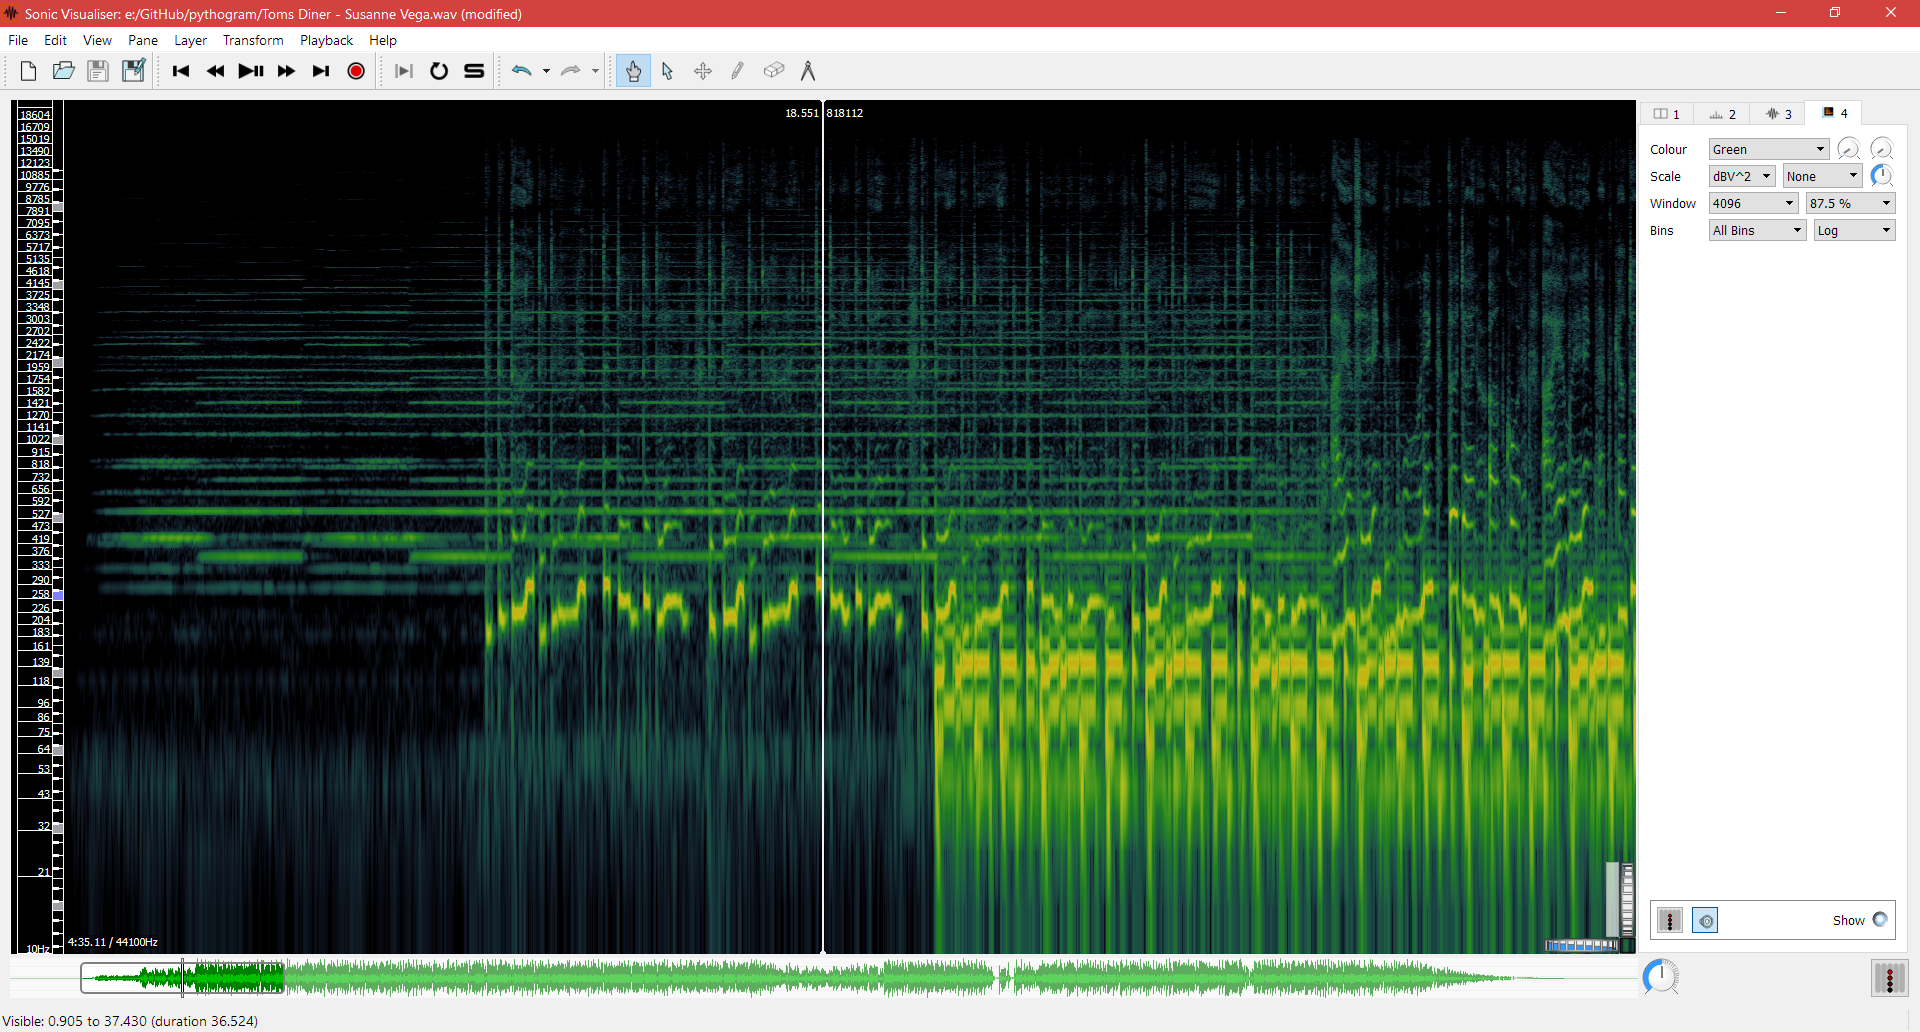
\includegraphics[width=1.0\textwidth]{Sonic_Toms_Diner_Spectrogram_close.png}
        \caption{Spektrogramm am Anfang des Songs "`Toms Diner"' in "`Sonic Visualiser"'}
    \end{minipage}
\end{figure}
\newpage
\subsection{Spek}\label{subsec:spek}

Mit dem kleinen Tool "`Spek"' kann man lediglich Audiodateien einlesen, deren Spektrogramm dann dargestellt wird. Leider gibt es bis auf die Sprache keinerlei Einstellungen. Man kann auch weder zoomen noch die Skalierung ändern. Das mag wohl daran liegen, dass diese Software zwischen 2010 und 2013 entwickelt wurde und sich immer noch in der Version 0.8.2 befindet.\\
Dennoch kann man damit sehr schnell sämtliche Audiosignale analysieren, was für einen ersten kurzen Eindruck des Signals vollkommen genügt.\vspace{2em}
\begin{figure}[H]
    \centering
    \begin{minipage}{1.0\textwidth}
        \centering
        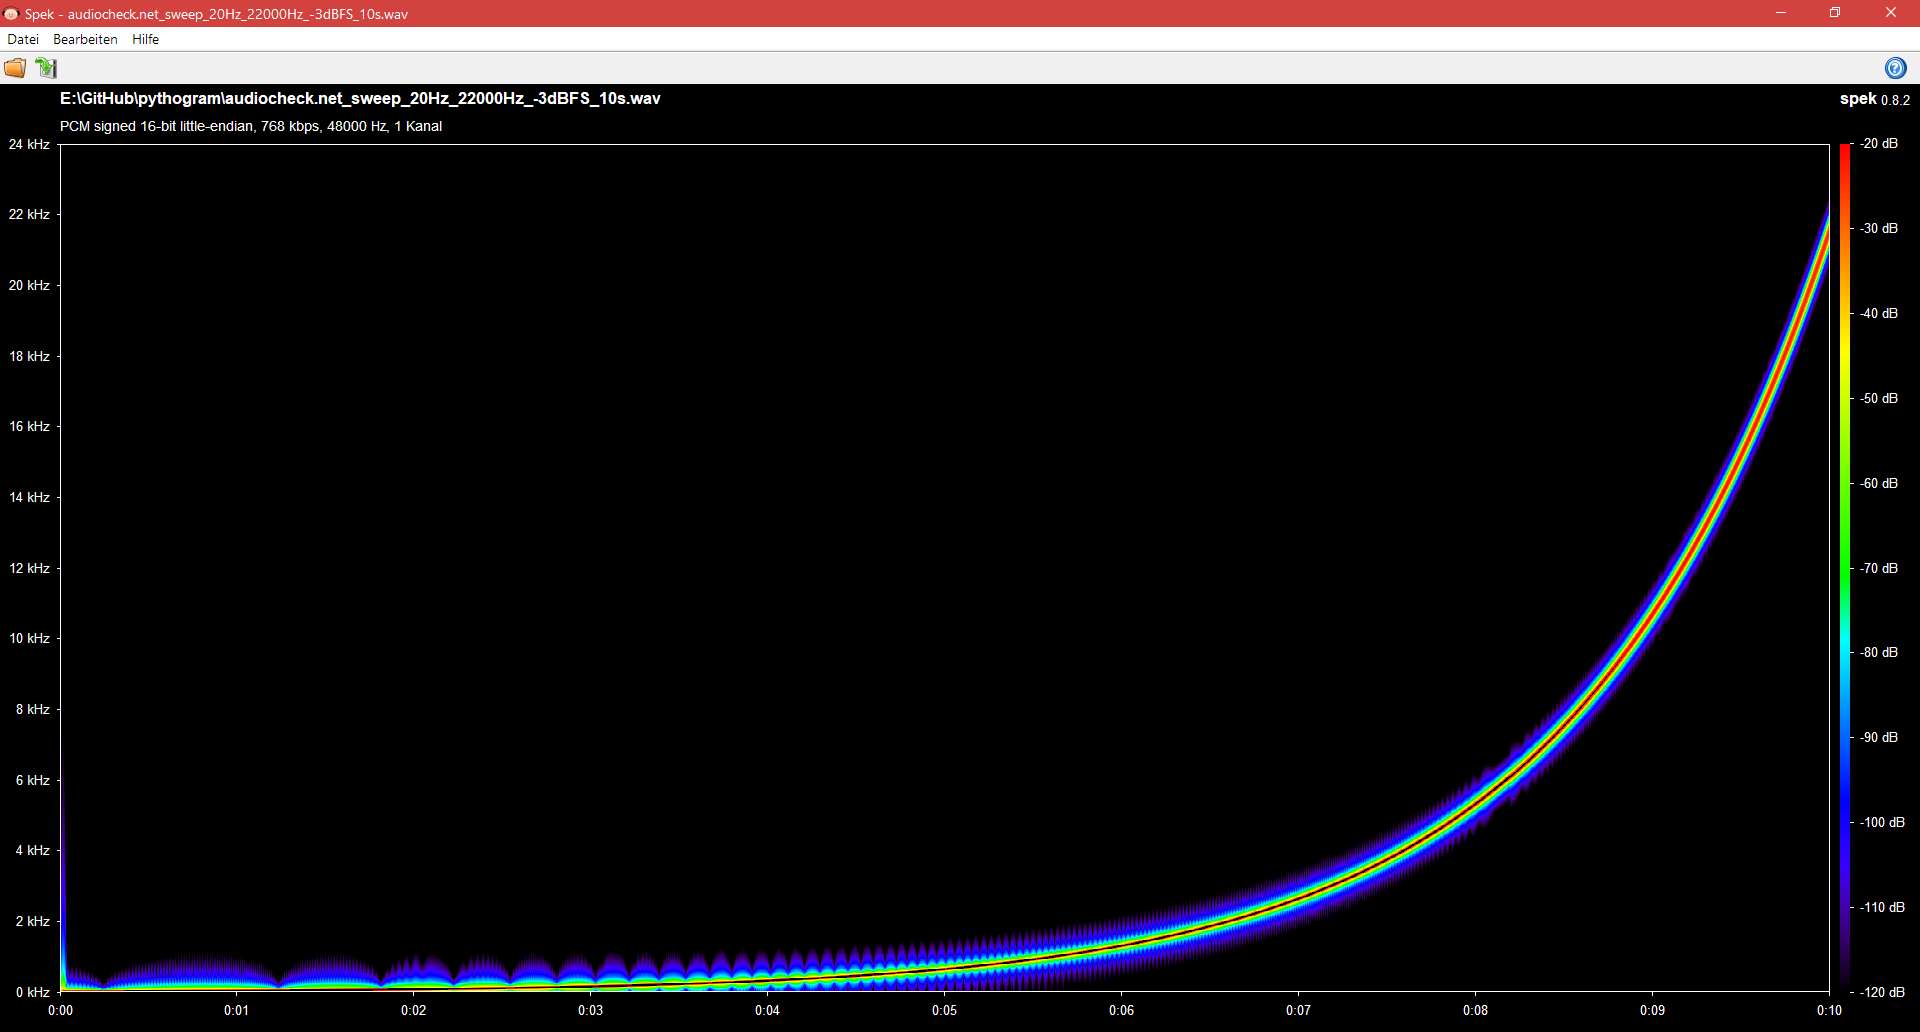
\includegraphics[width=0.8\textwidth]{Spek_Sine_Sweep.png}
        \caption{Steigender Sinus in "`Spek"'}
    \end{minipage}\hfill
\end{figure}
\begin{figure}[H]
    \centering
    \begin{minipage}{1.0\textwidth}
        \centering
        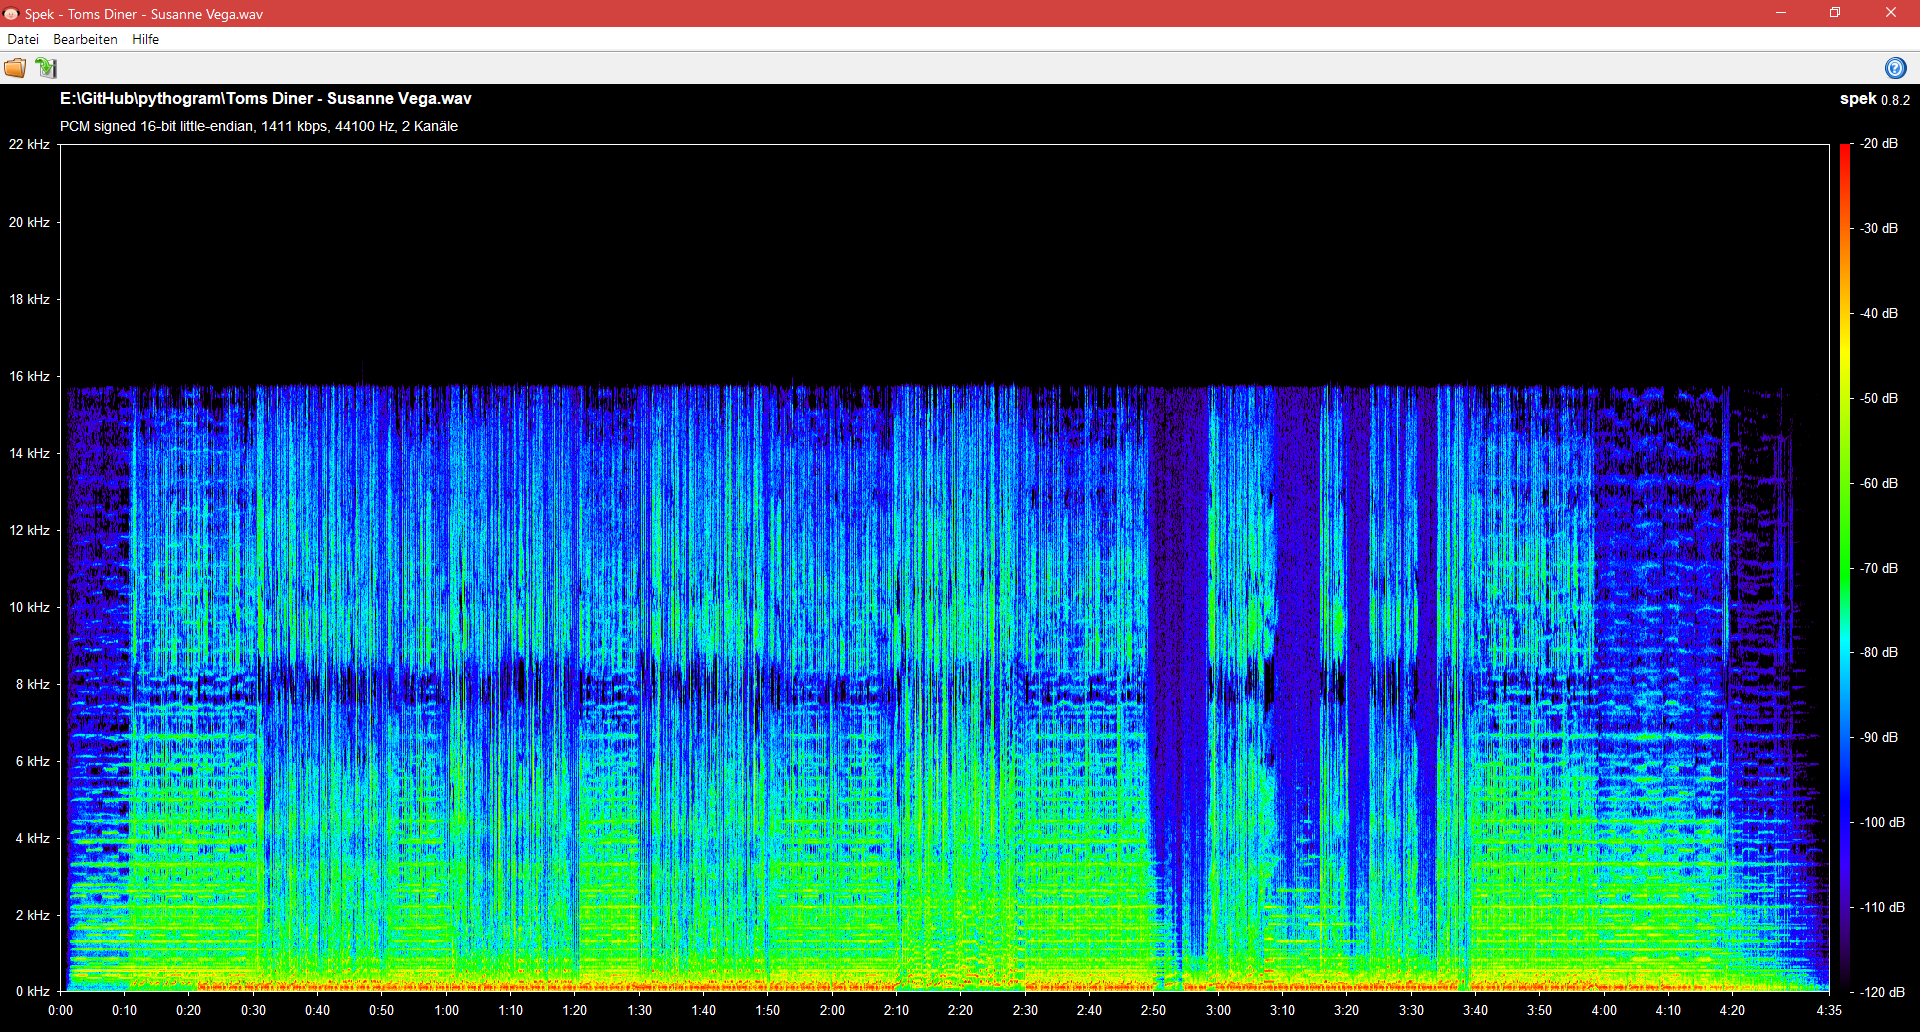
\includegraphics[width=1.0\textwidth]{Spek_Toms_Diner.png}
        \caption{Song "`Toms Diner"' - Susanne Vega in "`Spek"'}
    \end{minipage}
\end{figure}
\newpage
\section{Konzeption}\label{sec:konzeption}

\subsection{Anwendung}\label{subsec:anwendung}

\subsubsection{Benutzeroberfläche}

Ein konkretes Konzept für eine Benutzeroberfläche liegt nicht vor, da es zum Teil Bestandteil der Aufgabe und eine kleine Herausforderung für sich ist, Diagramme ordentlich darstellen zu können. Im Allgemeinen ist aber zu sagen, dass die Oberfläche übersichtlich und nicht zu überladen erscheinen soll.\\
Die Funktionen in den Anforderungen lassen sich möglicherweise gut auf einen einzelnen Screen platzieren. Sofern noch weiterreichende Funktionen implementiert werden, gilt es zu überlegen, wie diese eingebettet werden.

\subsubsection{Eingabeparameter}

Folgende Parameter sollen eingegeben werden können:
\begin{itemize}
  \item Signalerzeugung:
  \begin{itemize}
    \item Frequenz in Hz
    \item Abtastfrequenz in Hz
    \item Länge in s
    \item Amplitude
  \end{itemize}
  \item FFT-Auflösung
  \item Bandpass-Filter:
  \begin{itemize}
    \item untere Cutoff-Frequenz
    \item obere Cutoff-Frequenz
  \end{itemize}
  \item anzuzeigender Zeitbereich (Start und Ende)
\end{itemize}

\subsubsection{Darstellungsformen}

Die eingebenen Signale sollen laut Anforderung mindestens als Spektrum und als Spektrogramm dargestellt werden. Zudem möchten wir das Signal als Wellenform im Zeitbereich darstellen. Falls möglich soll die Ansicht auf die Diagramme verändert und die Diagramm(-ausschnitte) selbst auch als Bilder exportiert werden können.

\subsection{Testsignale}\label{subsec:testsignale}

Dem Nutzer soll es möglich sein, verschiedene Testsignale zu generieren und die entsprechenden Diagramme dazu betrachten zu können. Als Testsignale kommen Sinus-, Rechteck-, Sägezahn- und Dreieck-Signal in Betracht sowie ein weißes Rauschen. Zusätzlich soll die Möglichkeit bestehen, ein eigenes Audiosignal einlesen zu können, wobei es zunächst ausreicht, sich auf WAVE-Dateien zu beschränken.

\subsection{Zusammenfassung}\label{subsec:zusammenfassung}

\newpage
\section{Umsetzung und Evaluation}\label{sec:umsetzungUndEvaluation}

\subsection{Ziele}\label{subsec:ziele}

Das Ziel des Projektes war es, diverse Techniken der Signalverarbeitung grundlegend kennenzulernen, oder bereits bestehendes Wissen zu vertiefen, und dieses Wissen mit konventionellen Werkzeugen in der Skriptsprache Python anzuwenden, wobei auch ein funktionales und grobes ansprechendes Design eines Fensters umgesetzt werden musste. Zudem sollten natürlich möglichst viele der Grundanforderungen erfüllt werden.

\subsection{Werkzeuge}\label{subsec:werkzeuge}

Als Werkzeuge zur Entwicklung sollten Python 2.7, die IDE PyCharm, aber auch die mathematischen Grundpakete SciPy und NumPy dienen. Zur Fensterdarstellung sollte wxPython verwendet werden, wobei MatPlotLib unterstützend für die Darstellung des Spektrums und Spektrogrammes eingesetzt werden soll. Zur Verwaltung des Quellcodes sollte das Versionsverwaltungssystem Git in Kombination mit der Online-Plattform GitHub eingesetzt werden.

\subsubsection{Versionsverwaltung}

Für die Versionsverwaltung wurde ein Repository unter https://github.com/Timtam/pythogram angelegt, in welchem die Entwicklung des Programmes durchgeführt wurde, um sich gegenseitig nicht zu behindern. Hierfür wurde das Programm Git verwendet, welche die Möglichkeit zur Verfügung stellt, Dateien unabhängig voneinander zu bearbeiten, ohne sich dabei gegenseitig zu behindern, aber auch, jegliche Änderung mit einer hilfreichen Meldung zu versehen, damit man im Nachhinein nachvollziehen kann, wer warum welche Änderung eingeführt hat.

\subsubsection{Signalverarbeitung}

Die interne Signalverarbeitung wurde mittels NumPy und SciPy realisiert. NumPy dient hierbei für die grundlegende Mathematik, wie beispielsweise das Verwalten der Signale, das durchführen grundlegender Rechenoperationen mit diesen, aber auch das Erzeugen von Sinus-Testsignalen. SciPy stellt die Funktionen zur Erzeugung einer FFT zur Verfügung, aber auch vorgefertigte Funktionen, um weitere Testsignale wie Sägezahn, Dreieck und Rechteck zu generieren.

\subsubsection{Darstellung}

Für die Darstellung wurde wxPython verwendet, um die Oberfläche darzustellen. Das Panel, welches das Spektrogramm anzeigt, wird mittels MatPlotLib unterstützend erzeugt, welches automatisch Zoom-Funktionalitäten, Skalen und Speicherautomatismen anbietet.

\subsection{Umgesetzte Anforderungen}\label{subsec:umgesetzteAnforderungen}

\subsubsection{Benutzeroberfläche}

Die Oberfläche hat im Moment noch nicht viel zu bieten. Es ist ein minimalistisches Panel vorhanden, auf dem der Nutzer verschiedene Parameter und Einstellungen eingeben kann sowie verschiedene Testsignale auswählen kann und zudem die Länge und Abtastrate der Signale ausgegeben wird, die bei eigenen ausgewählten Dateien nützliche Informationen darstellen.
\vspace{2em}
\begin{figure}[H]
    \centering
    \begin{minipage}{1.0\textwidth}
        \centering
        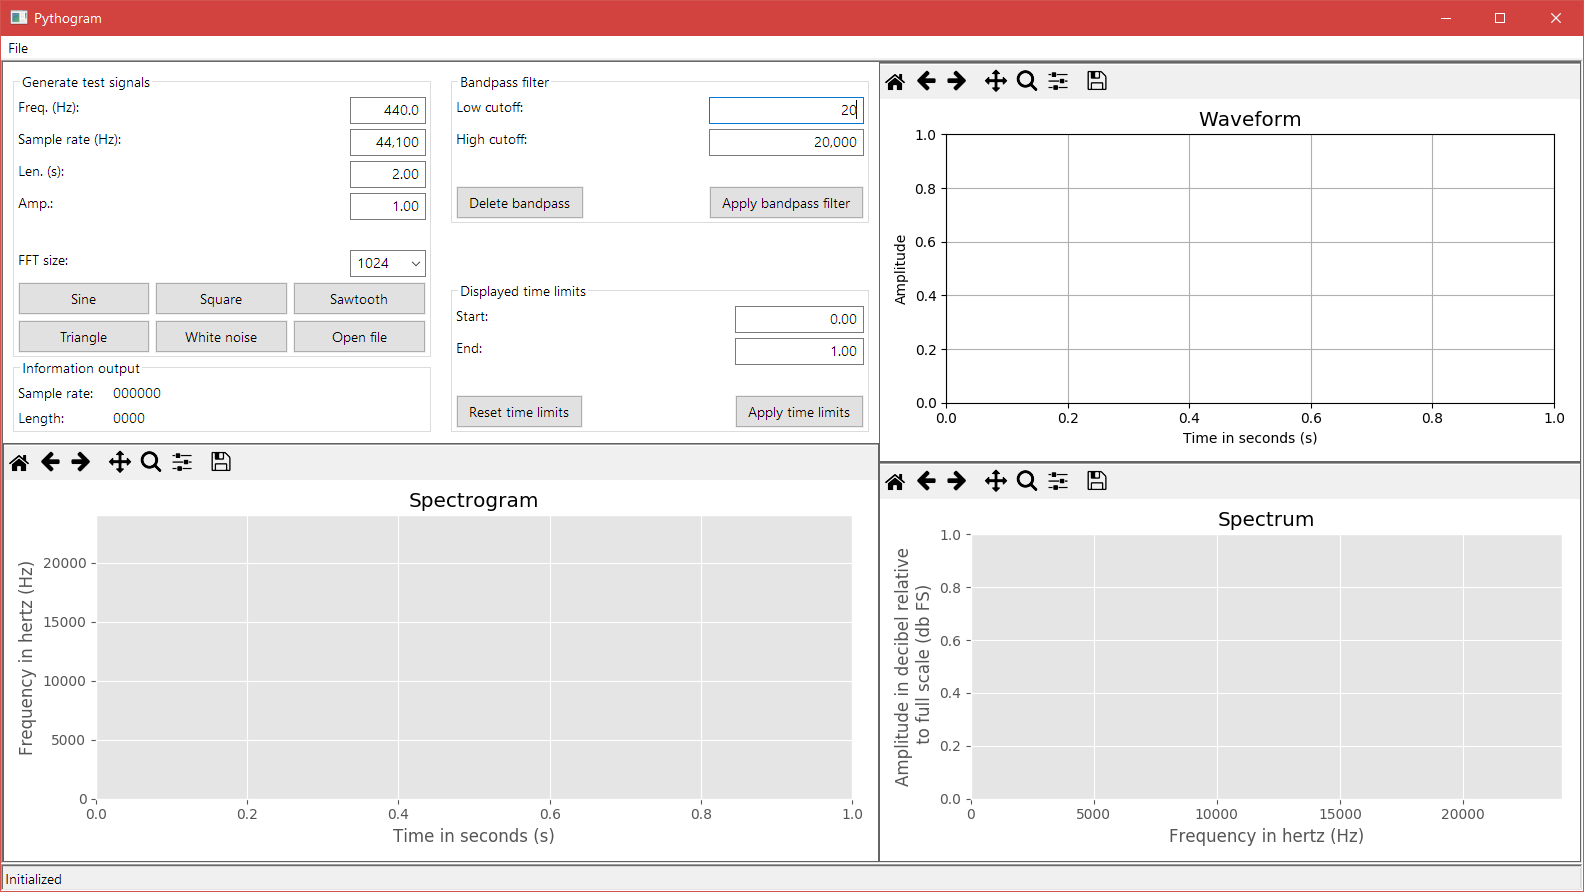
\includegraphics[width=1.0\textwidth]{GUI.png}
        \caption{Benutzeroberfläche von "`Pythogram"'}
    \end{minipage}
\end{figure}

\subsubsection{Darstellungen}

Die Anwendung realisiert 3 verschiedene Darstellungen von dem eingegebenen oder ausgewählten Signal. Das Diagramm in der oberen rechten Ecke zeigt die Schwingungen bzw. Amplituden des Signals über den Zeitbereich. Hierbei wird es standardmäßig auf den Bereich von 0 bis 1 Sekunde eingeschränkt, was man aber durch die Eingabe der Zeitgrenzen oder durch "`Bewegen"' im Diagramm selbst festlegen kann. Die y-Achse skaliert sich automatisch je nach dem, welche maximale oder minimale Amplitude im Signal vorkommt.\\
In der unteren rechten Ecke ist das Spektrum des gesamten Signals zu sehen. Dadurch sieht man, welche Frequenzen insgesamt im Signal vorkommen. Die Begrenzungen sind dabei auf der x-Achse die Frequenzen von 20 bis 24.000 Hz, wobei die Einteilung logarithmisch skaliert ist, und auf der y-Achse die Stärke der jeweiligen Frequenzen in dB relativ zur maximalen Amplitude (db FS) von -120 dB bis 0 dB. Das bedeutet, die am lautesten vorkommende Frequenz gibt den Bezugspunkt für alle anderen Frequenzen an, egal wie laut diese wirklich ist.\\
Im unteren linken Diagramm ist dann das Spektrogramm des gesamten Signals darstellt. Auch hier ist die y-Achse der Frequenzen mit den Begrenzungen von 20 bis 24.000 Hz initialisiert, die auch logarithmisch skaliert sind. Auf der x-Achse befindet sich dann die Zeit, die der Länge des Signals entspricht, und die Stärke der Frequenzen wird durch Farben dargestellt, die wiederum in dB FS angegeben sind.\vspace{1em}\\
In allen Diagrammen stehen zudem verschiedene Funktionen zu Verfügung.\\
Man kann die Standardansicht wiederherstellen (Haus), zwischen den Ansichten vor oder zurück wechseln (Pfeile), die Kurven oder Bilder in den Diagrammen verschieben (4-Pfeil-Kreuz), in sie hinein (Lupe + linke Maustaste) oder aus ihnen heraus zoomen (Lupe + rechte Maustaste), einige minimale Einstellungen am Layout vornehmen und den aktuellen Diagramm-Ausschnitt als Bild speichern.

\subsubsection{Testsignale und Evaluation}

Als Testsignale stehen sowohl Sinus, Rechteck, Sägezahn und Dreieck-Signale zur Verfügung, deren Frequenz, Länge und Sampling-Rate nach Belieben angepasst werden können. Außerdem kann ein weißes Rauschen erzeugt werden. Zudem kann jede Art von Wave-Dateien eingebunden werden, um auch eigene Signale in Pythogram betrachten und analysieren zu können. Das Signal wird dabei in jedem Fall in einen einzigen Audiokanal zusammengeführt, da mehrere Kanäle in Pythogram nicht separat analysiert werden können.\vspace{1em}\\
In den nächsten Abbildungen sind die verschiedenen Testsignal und die Diagramme zum Lied "`Toms Diner"' zu sehen.
\vspace{2em}
\begin{figure}[H]
    \centering
    \begin{minipage}{1.0\textwidth}
        \centering
        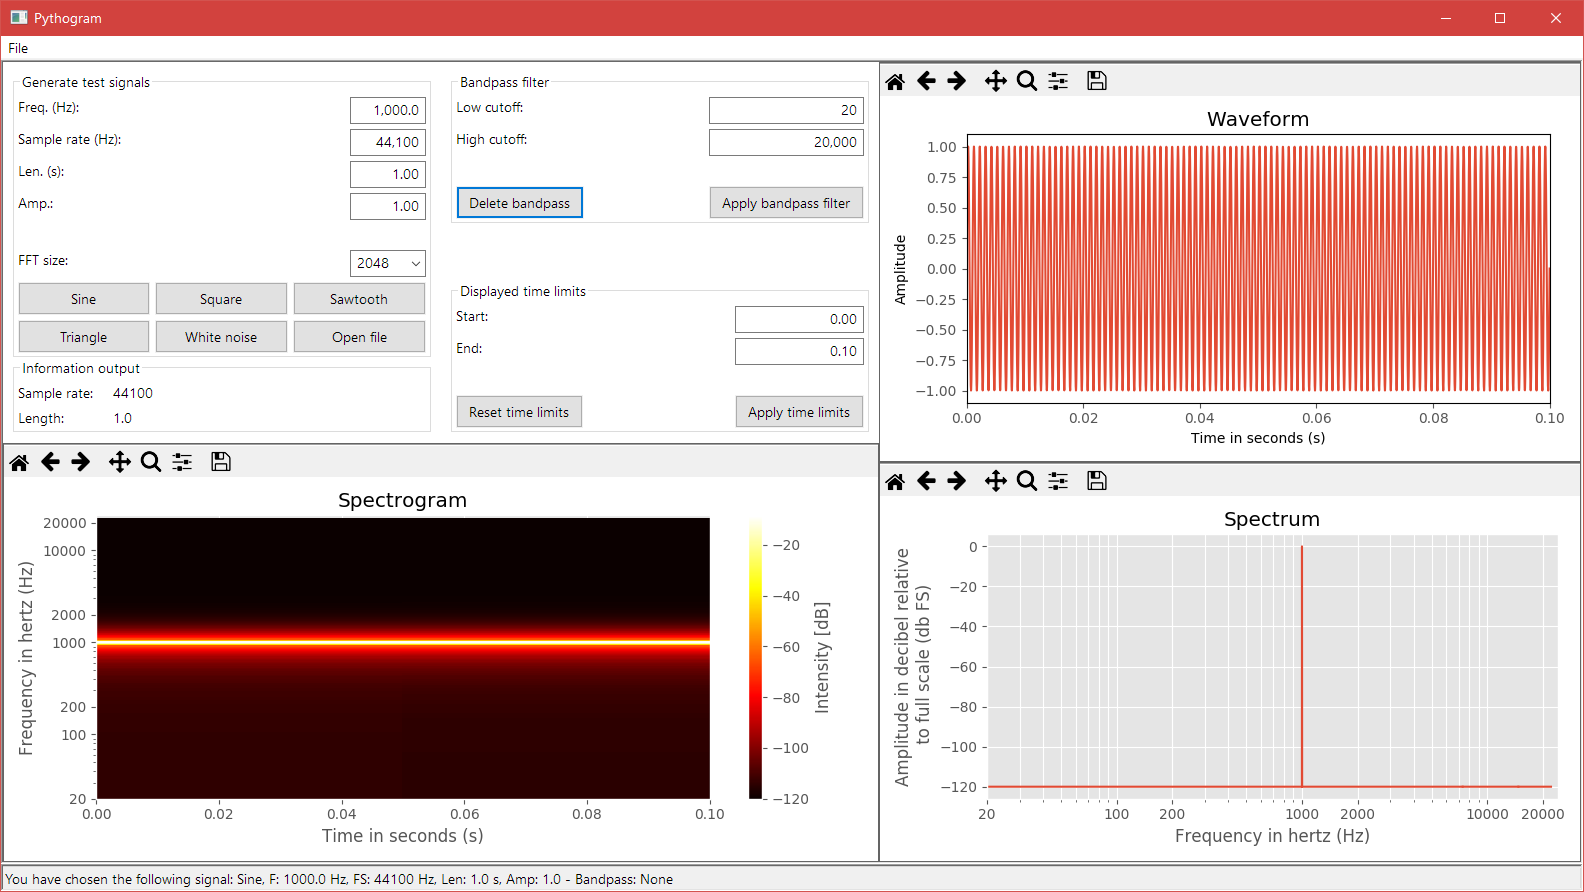
\includegraphics[width=1.0\textwidth]{Sine_1kHz.png}
        \caption{Sinus mit 1 kHz in "`Pythogram"'}
    \end{minipage}
\end{figure}
\begin{figure}[H]
    \centering
    \begin{minipage}{1.0\textwidth}
        \centering
        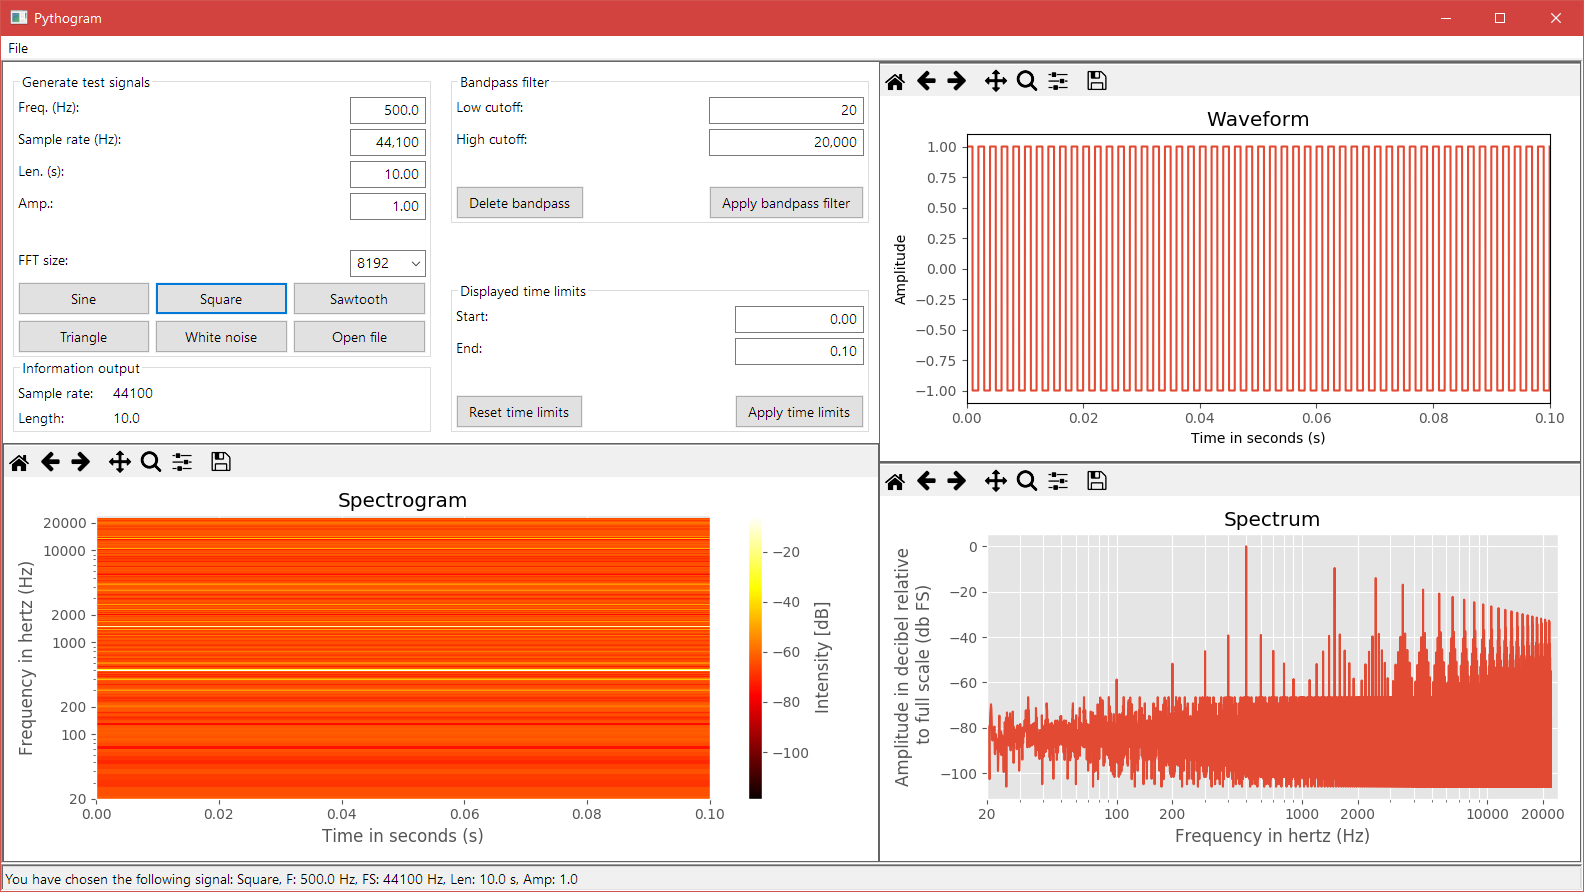
\includegraphics[width=1.0\textwidth]{Square_500Hz.png}
        \caption{Rechteck-Signal mit 500 Hz in "`Pythogram"'}
    \end{minipage}
\end{figure}
\begin{figure}[H]
    \centering
    \begin{minipage}{1.0\textwidth}
        \centering
        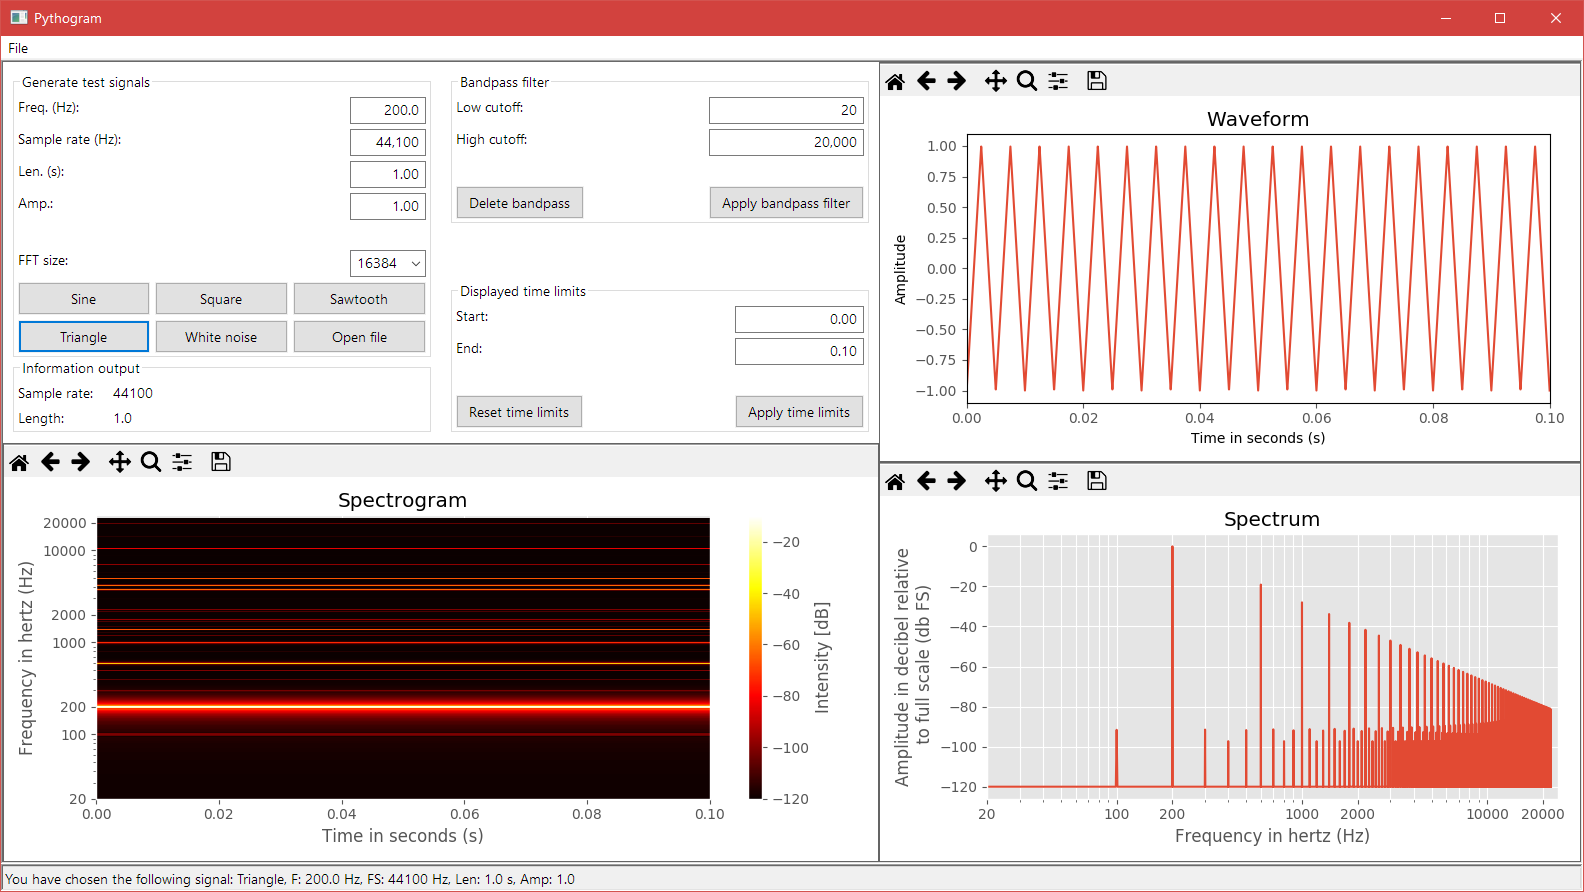
\includegraphics[width=1.0\textwidth]{Triangle_200Hz.png}
        \caption{Dreieck-Signal mit 200 Hz in "`Pythogram"'}
    \end{minipage}
\end{figure}
\begin{figure}[H]
    \centering
    \begin{minipage}{1.0\textwidth}
        \centering
        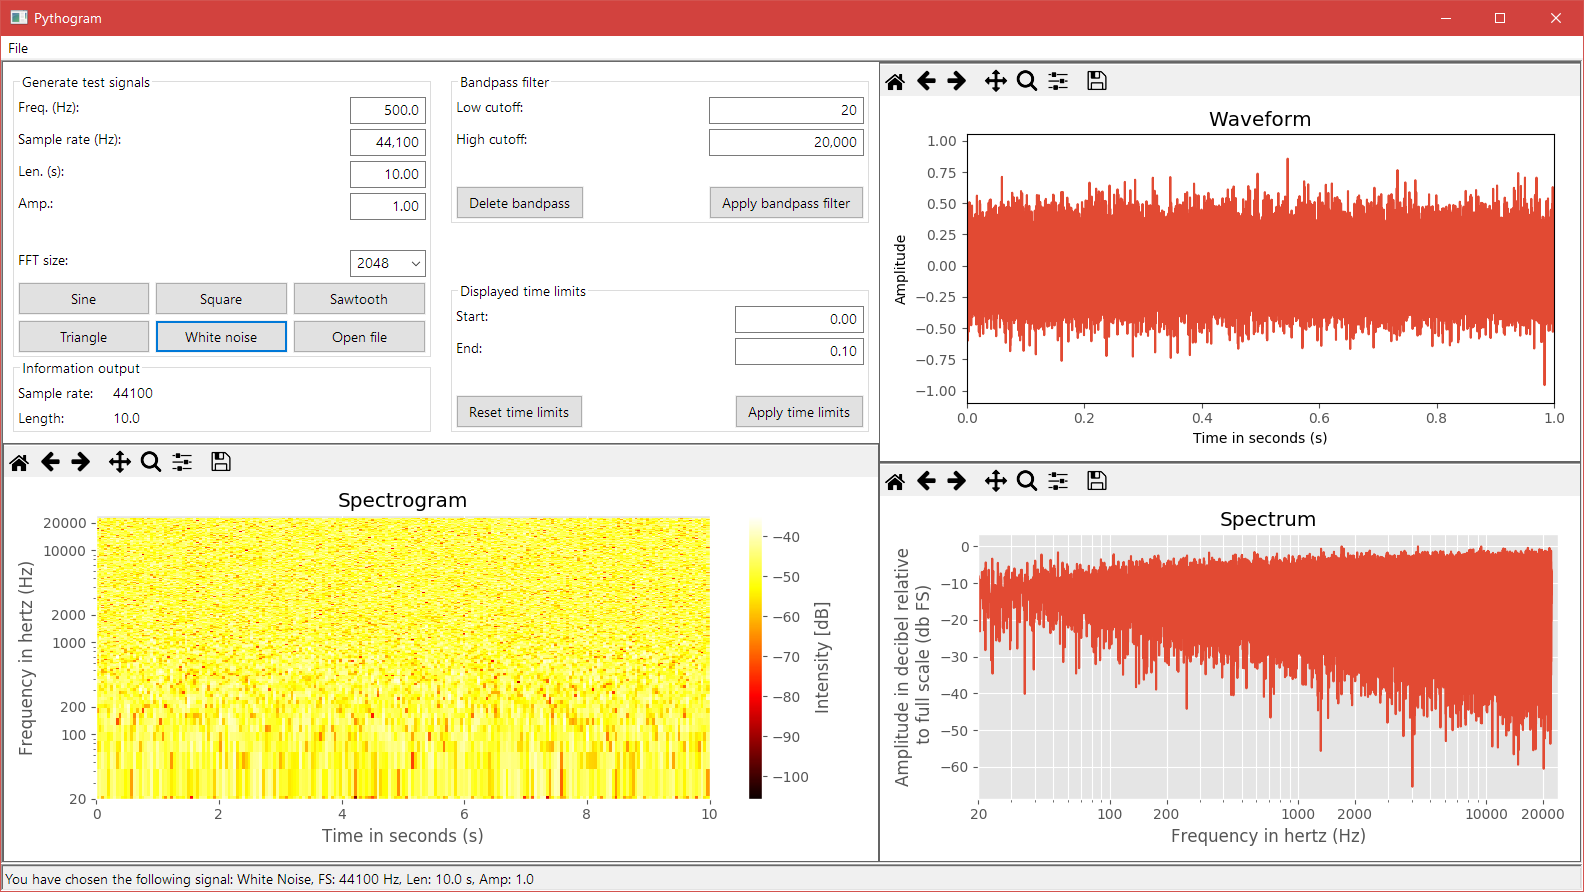
\includegraphics[width=1.0\textwidth]{WNoise.png}
        \caption{Weißes Rauschen in "`Pythogram"'}
    \end{minipage}
\end{figure}
\begin{figure}[H]
    \centering
    \begin{minipage}{1.0\textwidth}
        \centering
        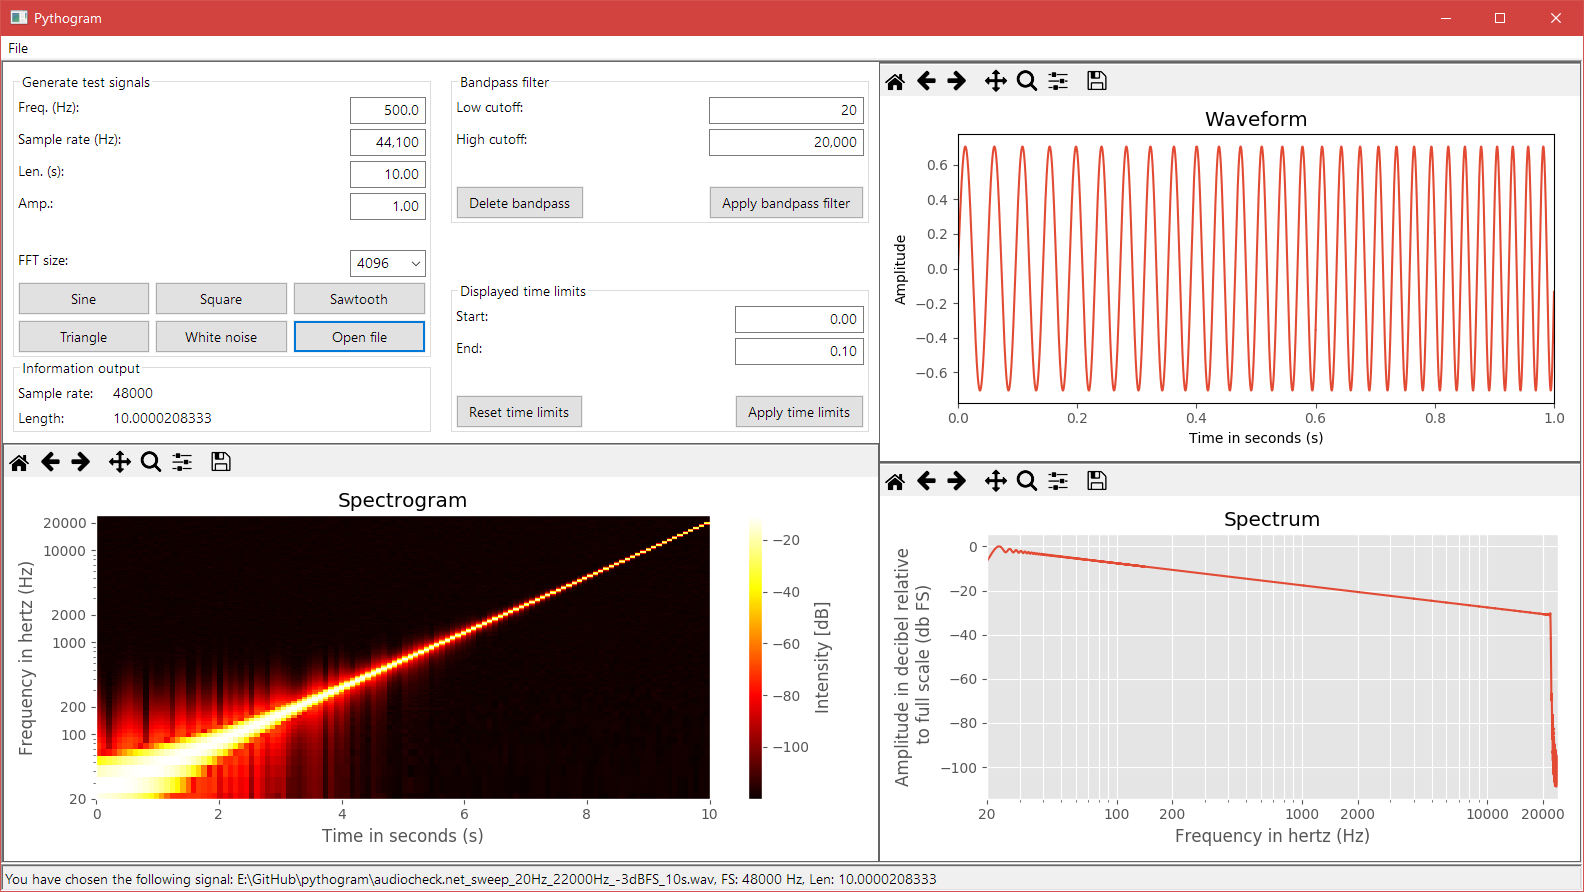
\includegraphics[width=1.0\textwidth]{Sine_Sweep.png}
        \caption{Steigender Sinus in "`Pythogram"'}
    \end{minipage}
\end{figure}
\begin{figure}[H]
    \centering
    \begin{minipage}{1.0\textwidth}
        \centering
        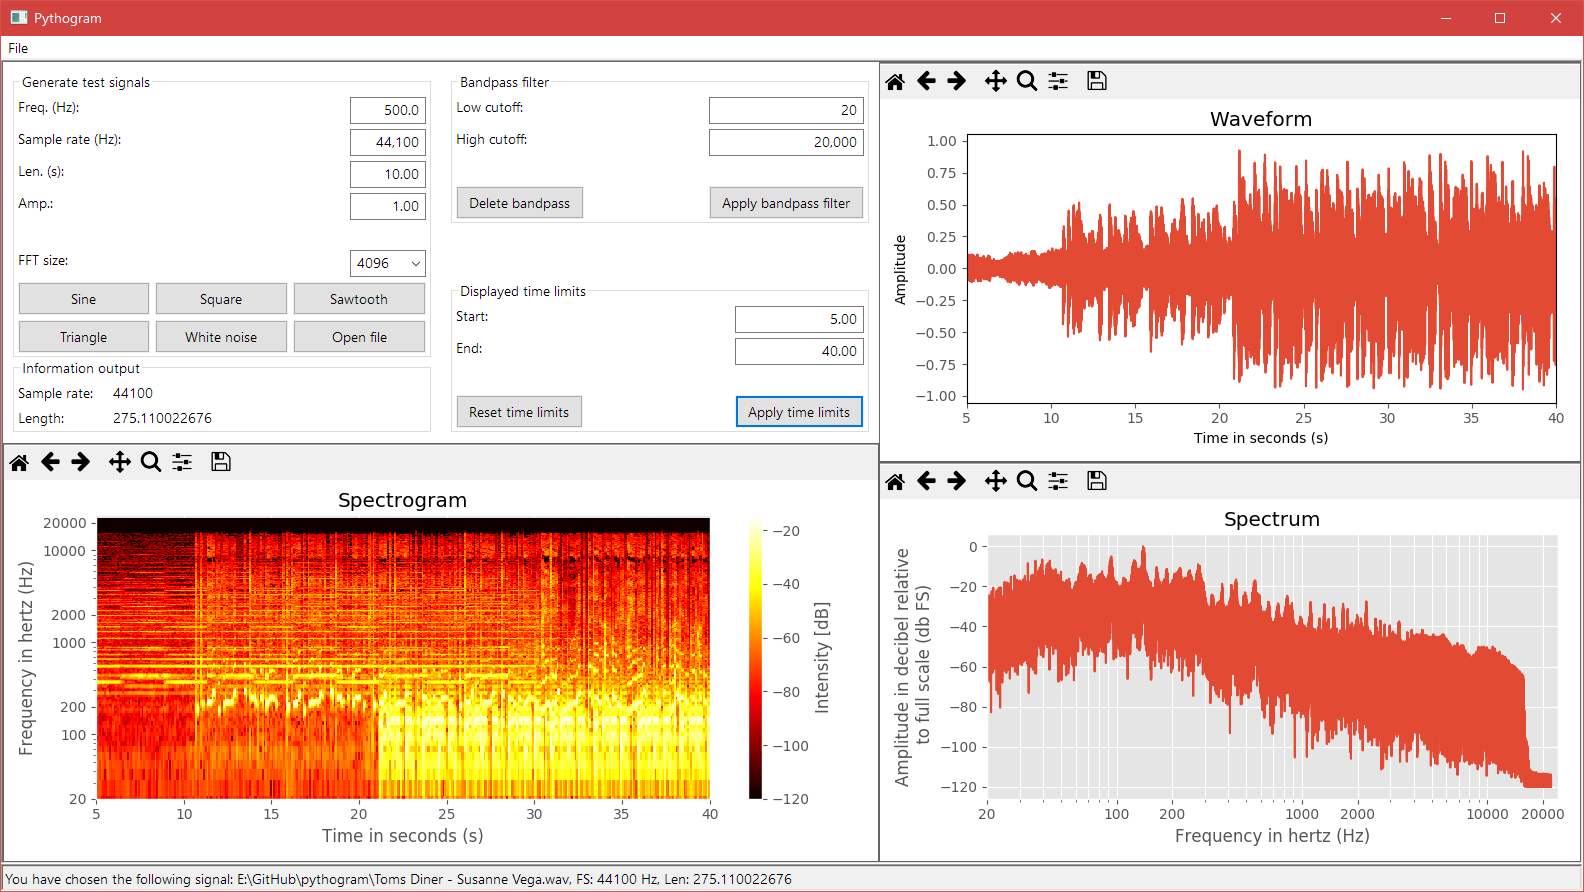
\includegraphics[width=1.0\textwidth]{Toms_Diner.png}
        \caption{Song "`Toms Diner"' in "`Pythogram"'}
    \end{minipage}
\end{figure}

\noindent
In der Abbildung des Spektrums eines einfachen Sinus-Signals kann man erkennen, dass die Darstellung des Spektrums richtig aussieht sowie auch die Darstellung im Spektrogramm. Bei den Rechteck- und Dreieck-Signalen ist in den Spektren die Tatsache, dass diese Signale aus mehreren Sinus-Signalen bestehen, gut zu erkennen und bekräftigt damit auch die korrekte Funktionsweise. Auch beim Rauschen sind alle Frequenzen im Durchschnitt gleich stark vertreten.\\
Vergleicht man nun die Spektrogramme des steigenden Sinus und des Lieds "`Toms Diner"', lassen viele Ähnlichkeiten feststellen und überzeugen daher auch von Korrektheit.\vspace{1em}\\
Die einzige Auffälligkeit bildet der harte Übergang zwischen den einzelnen vertikalen Spektren-Linien. Dies hätte durch eine Überlappung der Spektren zu einem einstellbaren Parameter wie im Programm "`Sonic Visualizer"' (Prozentzahl hinter "Window") reduziert werden können, wurde aber im Anbetracht des Aufwands und der zur Verfügung stehenden Zeit ausgelassen und war auch keine konkrete Forderung.

\subsection{Bandpass-Filter}

Die Funktionsweise der Bandbegrenzung wurde folgendermaßen überprüft: Es wurde ein Dreieck-Signal erzeugt, das bekanntlich Obertöne hat und damit aus mehreren Sinus-Frequenzen besteht. Stellt man die Begrenzungen nun ziemlich nah an die eingestellte Frequenz, bleibt nach der Filterung ein Signal zurück, dass ziemlich nah an einen Sinus heran reicht. Die folgenden Abbildungen bezeugen dies.\vspace{2em}
\begin{figure}[H]
    \centering
    \begin{minipage}{1.0\textwidth}
        \centering
        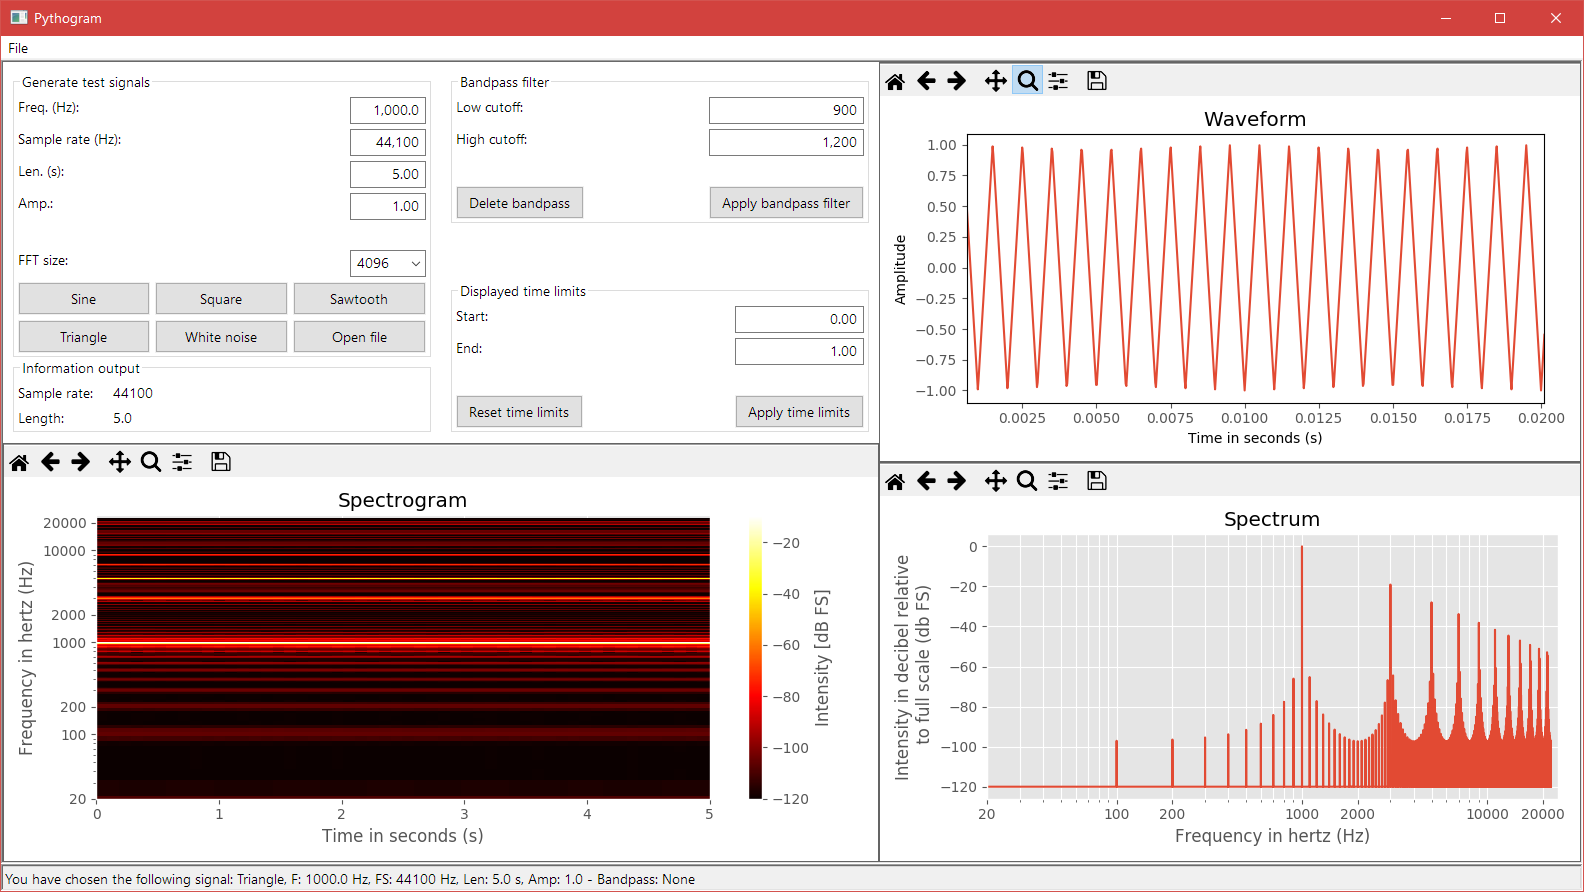
\includegraphics[width=1.0\textwidth]{Bandpass_Triangle.png}
        \caption{Dreieck-Signal mit 1 kHz in "`Pythogram"'}
    \end{minipage}
\end{figure}
\begin{figure}[H]
    \centering
    \begin{minipage}{1.0\textwidth}
        \centering
        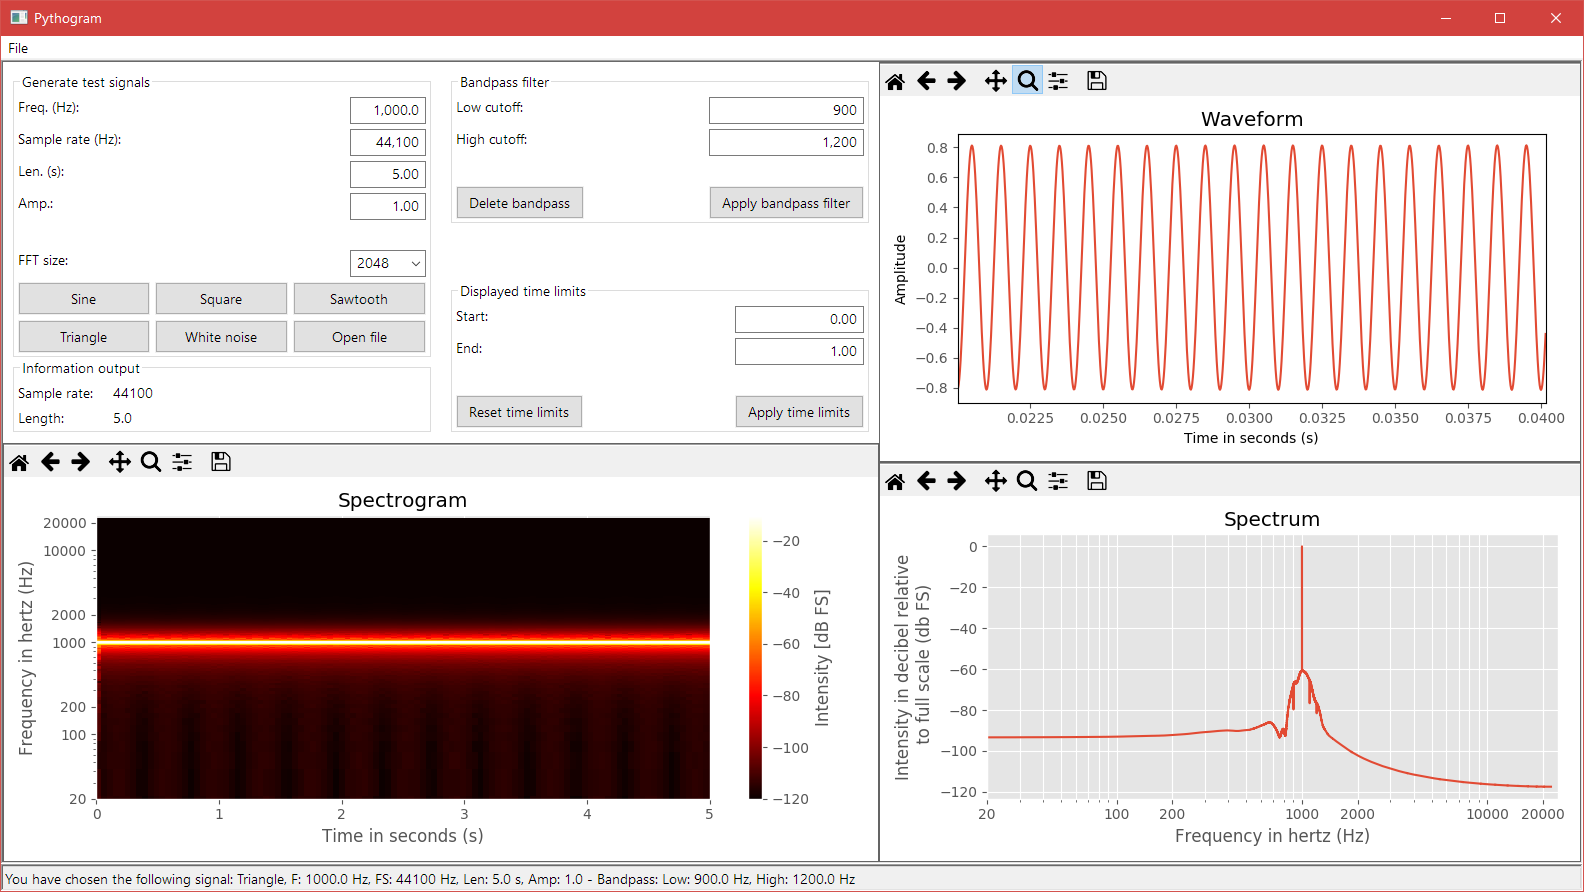
\includegraphics[width=1.0\textwidth]{Bandpass_Triangle_to_Sine.png}
        \caption{Gefiltertes Dreieck-Signal (1 kHz) bei 900 Hz und 1200 Hz in "`Pythogram"'}
    \end{minipage}
\end{figure}
\begin{figure}[H]
    \centering
    \begin{minipage}{1.0\textwidth}
        \centering
        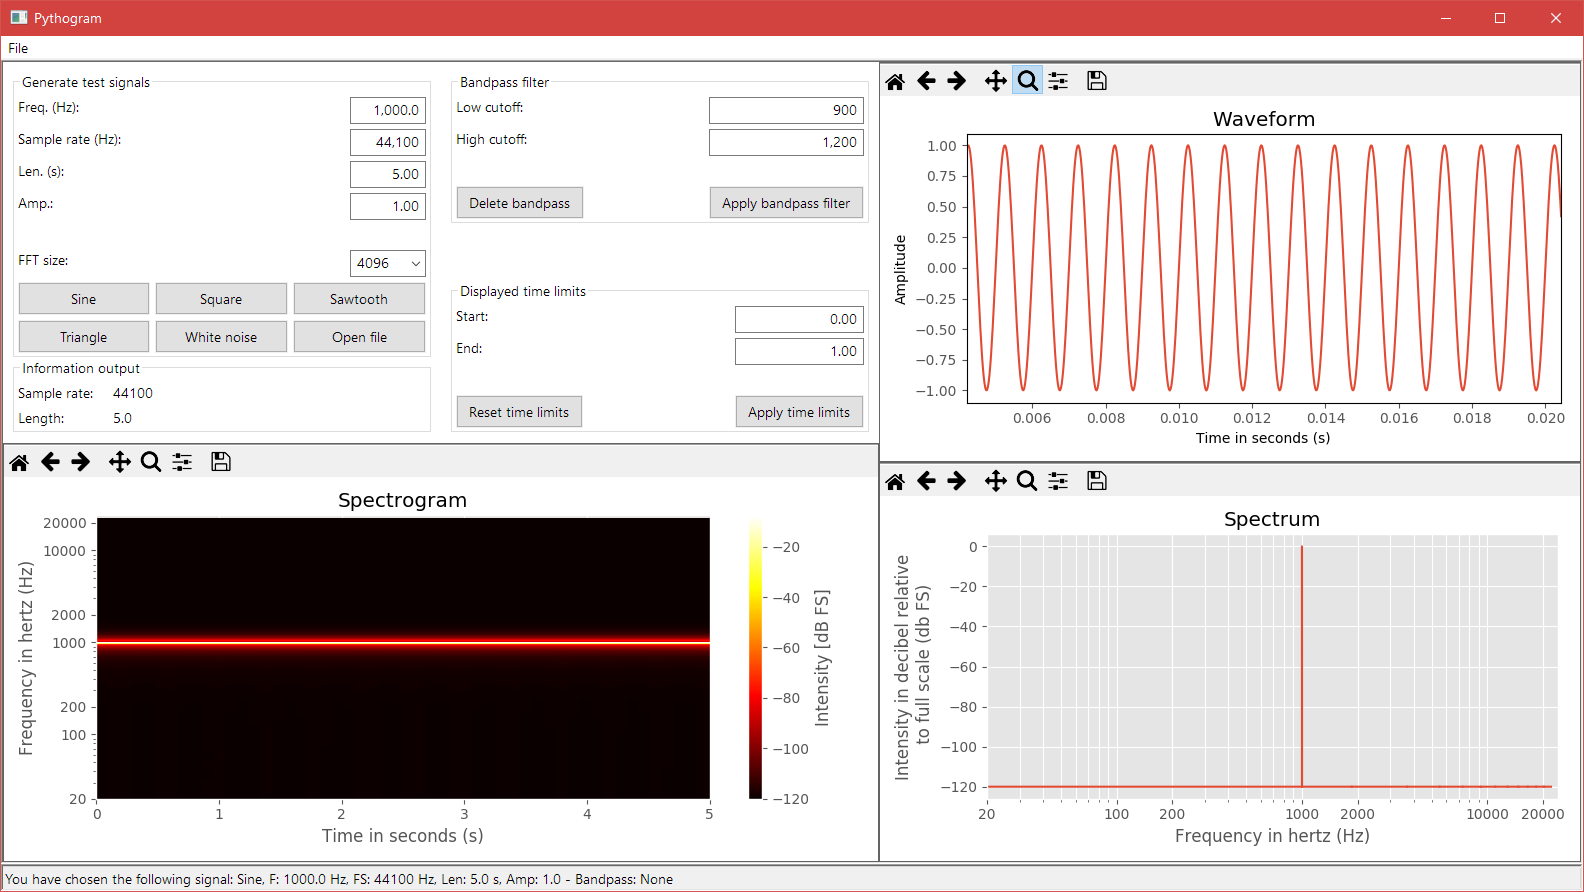
\includegraphics[width=1.0\textwidth]{Bandpass_Sine.png}
        \caption{Sinus mit 1 kHz in "`Pythogram"'}
    \end{minipage}
\end{figure}
\noindent
Zudem ist auch im Spektrum sehr gut ersichtlich, wie der Filter bei den Frequenzen agiert und an den eingestellten Frequenzen die Amplituden versucht, abzuschwächen.

\subsection{Zusammenfassung}\label{subsec:zusammenfassung2}

\newpage
\section{Zusammenfassung und Ausblick}\label{sec:zusammenfassungUndAusblick}

\end{document}